\documentclass[12pt]{book}
\usepackage[utf8]{inputenc}
\usepackage{graphicx}
\usepackage[a4paper,width=150mm,top=25mm,bottom=25mm,bindingoffset=6mm]{geometry}
\usepackage[utf8]{inputenc}
\usepackage[T1]{fontenc}
\usepackage[english]{babel}
\usepackage{setspace}
\usepackage{amsmath}
\usepackage{amssymb}
\usepackage{amsfonts}
\usepackage{bm}
\usepackage{fancyhdr}
\usepackage[round]{natbib}
\usepackage{algorithmic}
%\usepackage[noend]{algpseudocode}
\usepackage[backref = page]{hyperref}
\usepackage{color}
\usepackage{fancyvrb}
\usepackage{stmaryrd}
\usepackage{booktabs}
\usepackage{caption}
\usepackage{subcaption}
\usepackage{float}

\graphicspath{{images/}}

\newenvironment{acknowledgements}%
    {\cleardoublepage\null\vfill\begin{center}%
    \bfseries Acknowledgements\end{center}}%
    {\vfill\null}

\newenvironment {abstract}%
 {\cleardoublepage\thispagestyle{empty}\null\vfill\begin{center}%
    \bfseries\abstractname\end{center}}%
    {\vfill\null}

\newcommand{\fncyfront}
{
\fancyfoot [R]{}
\fancyhead [L]{\footnotesize {\leftmark}}
\fancyfoot [C]{\thepage}
\fancyhead [R, L]{}
\renewcommand {\headrulewidth}{0.0 pt}
}
%
%
\newcommand {\fncymain}{%
\fancyhead [R]{{}}
\fancyhead [L]{{\footnotesize \leftmark}}
\fancyfoot [C]{\thepage}
\fancyfoot [R]{}
\fancyfoot [L]{}
\renewcommand {\headrulewidth }{0.3 pt}
}
%
\setlength{\headheight}{14.5pt}
%
%
\begin{document}
\pagestyle{fancy}
\onehalfspacing
%
% header
\fncyfront
\frontmatter
\begin{titlepage}
%
\begin{center}
\begin{figure}[htbp]
\centering

\includegraphics[width=0.3\textwidth]{Images/unige2.jpg}
\end{figure}
%
{\LARGE University of Genoa\\}
%
%
{\Large {Department of Computer Science, Bioengineering,\\ Robotics and System Engineering}\\}
%
\vspace{0.7cm}
%
{\LARGE {Master Degree in Computer Engineering}\\}
%
\vspace{0.8cm}
%
%\rule{\textwidth}{1pt}
%
%
{\Huge \textbf{Verification and repair of machine learned controllers: a case study in prosthetics}\\}
%
%
\vspace{1.0cm}
%
\end{center}
%
\begin{minipage}{\textwidth}
\begin{flushright}
{\Large{ \bfseries Candidate}\\[0.1cm]
Dario \textsc{Guidotti}}
\end{flushright}
\end{minipage}
\\[1cm]
%
\begin{minipage}{0.5\textwidth}
\begin{flushleft}
{\Large
{\bfseries Advisor}\\[0.1cm]
Prof. Armando \textsc{Tacchella}}
\end{flushleft}
\end{minipage}
\\[0.4cm]
\begin{minipage}{0.5\textwidth}
\begin{flushleft}
{\Large
{\bfseries Co-advisor}\\[0.1cm]
Prof. Claudio \textsc{Castellini}}
\end{flushleft}
\end{minipage}
%
\vfill
\begin{center}
{\Large August, 22nd 2018}
\end{center}
\end{titlepage}
\thispagestyle{empty}
\null \vspace {\stretch{1}}
        \begin{flushright}
        \emph{To all the people with whom I have been sharing \\ worries, success and happiness \\ during these years.}
        \end{flushright}
\vspace {\stretch{8}}\null
%
\newpage
%
\thispagestyle{empty}
\null \vspace {\stretch{1}}
        \begin{flushright}
        \emph{The greatest challenge to any thinker is stating \\ the problem in a way that will allow a solution.} \\% \rule{200pt}{0.4pt} \\ 
        Bertrand Russell
        \end{flushright}
\vspace {\stretch{8}}\null
\begin{abstract}
Myocontrol is a hot subtopic of assistive robotics, in particular it is one of the so-far unsolved hurdles in upper-limb prosthetics. It is about swiftly, naturally and reliably converting biosignals, non-invasively gathered from an upper-limb amputated subject, into control commands for an appropriate self-powered prosthetic device.
Despite decades of research, traditional surface electromyography cannot yet detect the subject's intent to an acceptable degree of reliability, that is, enforce an action exactly when the subject wants it to be enforced.\\\\
In this work we tackle one of the subproblems related to myocontrol reliability, namely activation overshooting, and show that Formal Verification can indeed be used to mitigate it at an acceptable computational cost. Eighteen intact subjects were engaged in two Target Achievement Control tests in which a standard myocontrol system was compared with two "repaired" ones, one using a simple non-formal technique, enforcing no guarantee of safety, and the other using Satisfiability Modulo Theories (SMT) technology to rigorously enforce it. The experimental results indicate that both repaired systems exhibit an improved reliability by reducing activation overshooting. Using the SMT-based system only requires a modest increase in the required computational resources.
\end{abstract}
\begin{acknowledgements}
HERE ACKNOWLEDGEMENTS
\end{acknowledgements}
%
\tableofcontents
\listoffigures
\listoftables

\fncymain
\mainmatter
\chapter{Introduction}\label{c:introduction}
\section{Context}\label{sec:context}
As testified in \cite{ZIEGLERGRAHAM2008422} "One in 190 Americans is currently living with the loss of a limb. Unchecked, this number may double by the year 2050": this kind of statistic can easily express how much prosthetic technologies are important nowadays and how big is the market for them.
By virtue of the above-mentioned high demand of prosthesis, technological research in the prosthetic domain in the last decades has been very active: ideally amputees would need, as far as possible, prosthesis as functional as real limbs and a great deal of research as been done to try to enhance the performance, the comfort and the appearance of prosthetic limbs. Sadly, even with all the effort done from the scientific community, we are still far from developing this kind of prosthetic limbs: in particular, even if relatively dexterous prostheses are commercially available, reliable prosthetic control is still an open problem. As testified in \cite{castellini2016upper}, detecting the patient's intent and transforming it into effective control signals is still a largely open problem. During the last few years machine learning has become more and more common as control method: various machine learning model has been used to extrapolate control policy from data provided from disparate type of sensors.
One of the most commonly used sensor is the electromyographic (EMG) sensor, which allows to measure the electrical activity of muscles: this kind of sensor owes its popularity to its (relatively) low cost and to the fact that it can be used without the need of invasive surgical procedures. Although the control methods for prosthesis using EMG signals are constantly improving, from \cite{Zecca2002} to \cite{Strazzulla2017}, the control system is still the bottleneck for the diffusion of machine learned controlled prosthesis in the daily life of the standard amputee: in particular the main problem of the current state of the art machine learned controller is the reliability, e.g. the ever-present possibility that the system will take the wrong decision, potentially leading to catastrophic results.
In the last years the interest in the reliability of machine learning system has increased more and more: in particular for safety critical application it is imperative to guarantee an high reliability and current machine learning systems are usually unable to guarantee it. One of the current state of the art methods used to enhance the reliability of machine learning system consist in leveraging formal methods in order to verify and eventually repair machine learning system. This kind of method has been mainly applied to neural networks system and a thorough presentation of its state of the art can be found in \cite{leofante2018automated}.
\section{Motivations}\label{sec:motivations}
As testified in \cite{biddiss2007upper} the mean rejection rate for electric prostheses is 35\% for the pediatric population and 23\% for the adult population and one of the critical factor for the rejection is the unsatisfactory state of the available technology [\cite{biddiss2007upperfact}].
In particular one of the lacking aspect pointed out in \cite{biddiss2007upperfact} and, more recently, in \cite{castellini2016upper} was the ease of control of the prostheses: whereas the machine learned controllers have grown more and more refined [\cite{Strazzulla2017}] the reliability of this kind of controllers is still the bottleneck for the passage from the research community to the industrial one.
The problem of the insufficient reliability of machine learning system has become increasingly interesting for the research community in the last few years: although machine learning systems are becoming more and more common in industrial application, they present limited application in safety/security critical domain due to their limited reliability. In order to enhance the reliability of machine learning systems the research community has tried different approaches: in particular we are interested in the approach which uses formal methods, and in particular formal verification, in order to analyse and eventually repair machine learning models. In \cite{leofante2018automated} a thorough presentation of the state of the art of the above mentioned approach can be found.
Even if the research done on this approach consider mostly neural networks as machine learning models of interest and, as far as we know, there hasn't been any temptative to apply this kind of methods in the domain of prosthesis control, we believe that the application of formal methods could truly enhance the reliability of our machine learned myocontroller and, consequently, improve the confidence on deploying the controller and lower the rejection rate.
\section{Goals}
In this thesis we are addressing the problem of studying if it is possible to enhance the reliability of the current machine learning models used to control prosthetic upper limbs by means of EMG signals. We will study an unresolved control problems in the system "Interactive MyoControl" currently used at the DLR and then we will try to use state of the art decision procedures, opportunely modified, to solve aforesaid problems, or at least to improve the present system.
We will then present the results obtained from an experiment we have designed in order to show the difference between the original control system and the enhanced version.
\section{Contributions}\label{sec:contributions}
In this work we study a open reliability problem in the control of prosthetic hands, we propose a computationally feasible algorithm for the enhancement of the reliability of the system with respect to the above mentioned problem and we show through experimental results that our algorithm indeed manages to limit the appearance of the above-mentioned problem.
\section{Overview}\label{sec:overview}
This thesis is structured as follows:

Chapter \ref{ch:background} briefly presents the background topics, such as an introduction to myoelectric control, formal methods, in particular formal verification, Satisfiability and Satisfiability Modulo Theories. Moreover we present the machine learning models of interest, in particular Ridge Regression (RR) and Ridge Regression with Random Fourier Features (RR-RFF).

Chapter \ref{ch:preliminaries} introduces the myocontrol system currently used at DLR, in particular the hardware used with the system and the most important characteristic of the interaction between the hardware and the software components. We also present the SMT solver we have decided to use in this work and its most important features.

Chapter \ref{ch:problem-definition} presents our formal definition of the problem of interest and how we have proceeded in our study in order to develop a feasible solution. We also show the structure of our algorithms and an example of execution of the same. We then explain the main differences between the different algorithms and their features.

Chapter \ref{ch:exp-result} presents the experiments we have designed in order to analyse the efficacy of our algorithms, it explains the choices we have made in the designing of the experiments and it shows the experimental protocol we have followed. Furthermore it presents the experimental results we have found from the statistical analysis of the data collected during the two experiments. 

Chapter \ref{ch:conclusion-future}  points out achieved results and future work directions.
\chapter{Background}\label{c:background}
In this chapter we introduce background notions and survey related work. To be specific section \ref{sec:EMG} briefly present myoelectric control, section \ref{sec:decproc} briefly presents formal methods and in particular the formal verification techniques we use in this thesis. Section \ref{sec:ML} presents the machine learning methods of interest.
\section{Myoelectric Control}\label{sec:EMG}
\begin{figure}[ht]
    \centering
    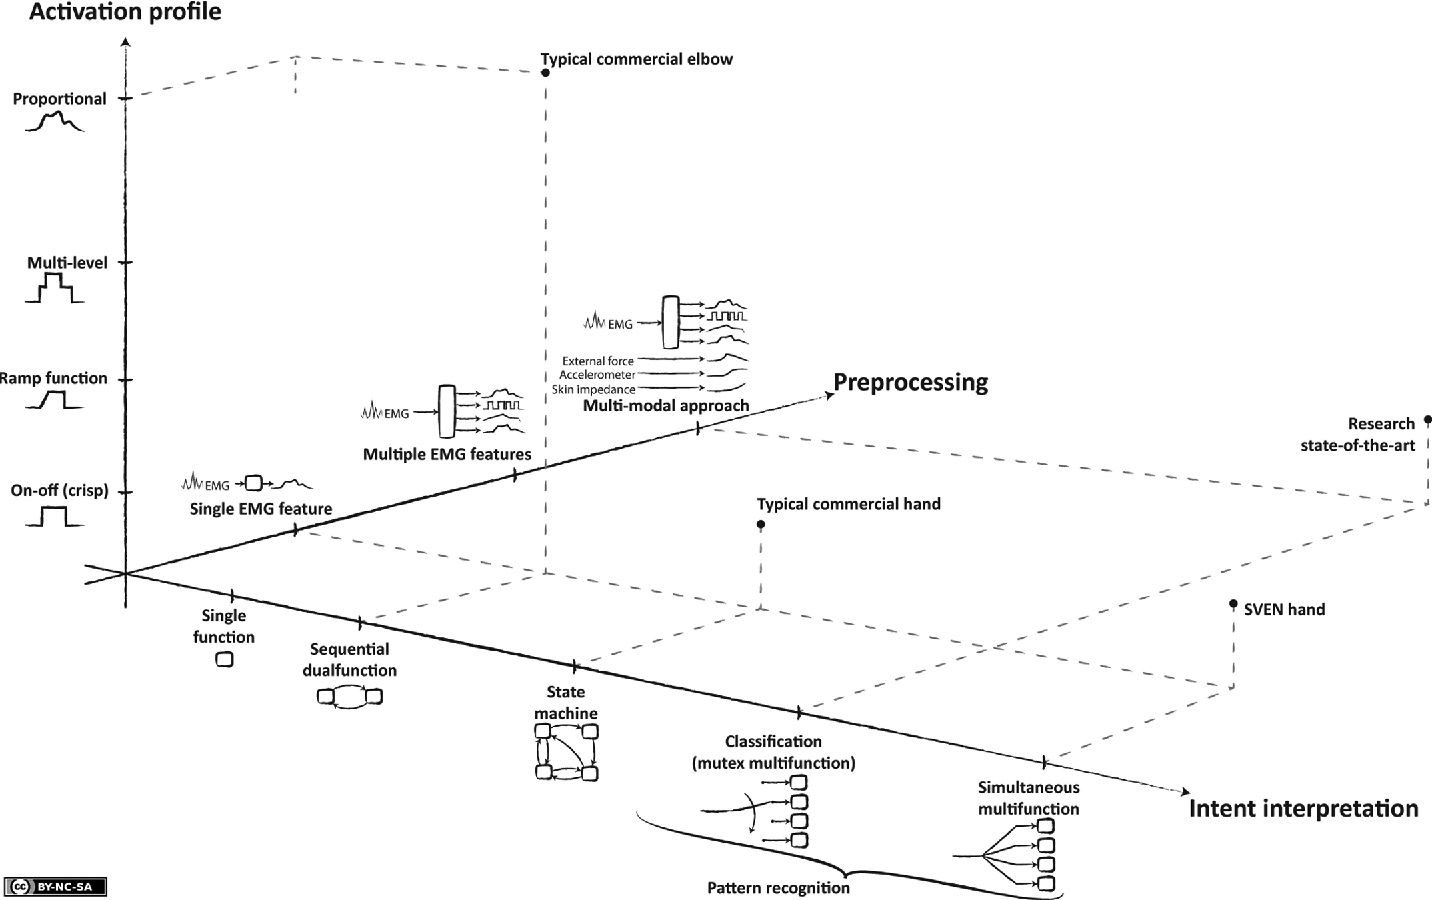
\includegraphics[width=1\textwidth]{Images/myoelectric-control.png}
    \caption{Research state-of-the-art of myoelectric control in the year 2012 [\cite{Fougner2012ControlOU}]}
    \label{fig:myo-control-schema}
\end{figure}
Electromyography (EMG) is an electrodiagnostic technique for evaluating and recording the electrical activity produced by skeletal muscles [\cite{0736093400}]. EMG is performed using an electromyograph which detects the electric potential generated by muscle cells when they are electrically or neurologically activated.
This electric potential can be approximatively considered proportional to the force of the muscle activation.
Due to the preference for noninvasive prostheses, surface EMG (sEMG) signals have been used for the control of upper limb prostheses prosthetic devices since 1948, as testified in \cite{Zecca2002}.
The signal produced by the sEMG sensors are fed to machine learning methods in order to control the prostheses: different machine learning models are used in union to different numbers of sEMG sigmals in order to achieve different level of control on the prostheses. A graphical representation of the different control methods and level, considering also non-machine learning methods, can be found in figure \ref{fig:myo-control-schema}.
In this thesis we work on a myoelectric control system characterized by a \textit{proportional} activation profile, a \textit{simultaneous multifunction} intent interpretation and we consider as input \textit{multiple EMG features}.
\section{Formal Methods}\label{sec:decproc}
Formal methods are a kind of system design techniques which use meticulous mathematical models for the specification, development and verification of software and hardware systems. The application of these kind of methods to the design of both software and hardware systems is supported by the increased reliability and robustness of the resulting systems. In this thesis we are more interested in the use of formal methods as verification techniques: we will consider a finished system and we will try to use the verification techniques in order to enhance its reliability.
In particular the system we will consider is a machine learned controller, therefore in this section we present two of the most popular formal verification techniques used in the verification of machine learning systems: Satisfiability (SAT) and Satisfiability Modulo Theories (SMT).
\subsection{Satisfiability (SAT)}
\begin{figure}[ht]
    \centering
    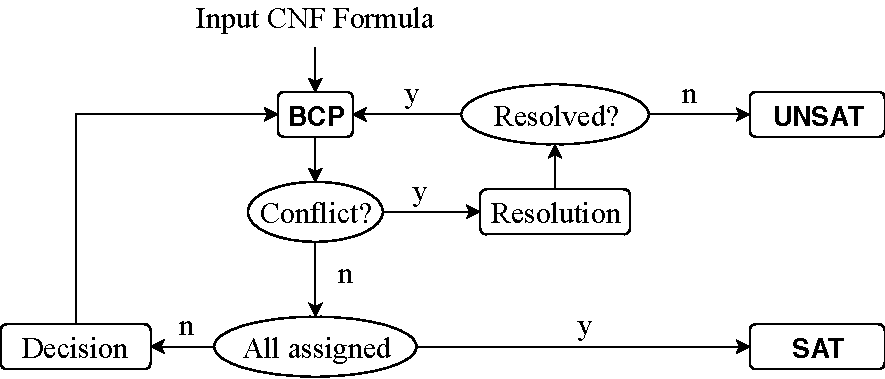
\includegraphics{Images/SAT.pdf}
    \caption{The CDCL framework.}
    \label{fig:cdcl-frame}
\end{figure}
SAT solving aims to check the satisfiability of a propositional logic formula $\varphi$ represented as Boolean combinations of atomic (Boolean) propositions. We introduce CDCL-style SAT solving algorithm, being the most commonly implemented in state-of-the-art SAT solvers.
The CDCL algorithm starts from a CNF formula and then explores the search space by iteratively assigning truth values to some propositions which are chosen according to some heuristic. After each of these assignment the algorithm applies Boolean Constraint Propagation (BPC) to determine the variable assignments implied by the last decision. If the application of BPC leads to a conflict, which is, if the value of a variable is implied to be both true and false at the same time, then \textit{conflict-driven clause-learning} and \textit{non-chronological backtracking} are employed: the algorithm follows back the chain of implication and applies resolution to infer a reason for the conflict in the form of a conflict clause, which then is added to the clause set of the solver. Backtracking removes previous decisions and their implications until the conflict clause can be satisfied. If the starting CNF formula has clauses consisting of a single literal, the algorithm assign them directly. As consequence the algorithm starts with BCP in order to detect implication. If the application of BCP brings to a conflict, the algorithm tries to resolve such conflict. If the conflict is unsolvable then the CNF formula is unsatisfiable, otherwise the algorithm backtracks and continues with BCP. If BCP is completed without conflicts and there are still unassigned propositions, the algorithm makes a new decision. Otherwise the CNF formula is satisfiable and a solution is found.
%
\subsection{Satisfiability Modulo Theories (SMT)}
\begin{figure}[ht]
    \centering
    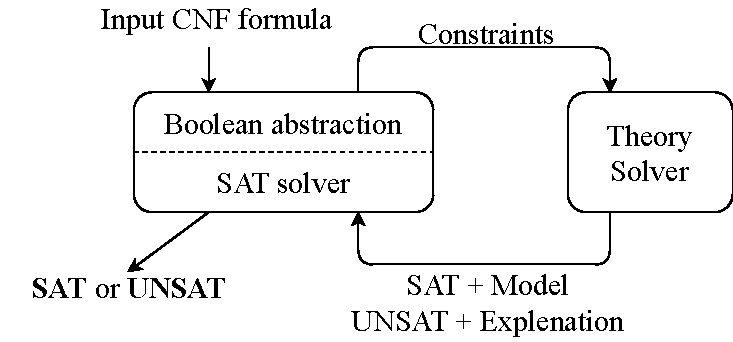
\includegraphics{Images/SMT.pdf}
    \caption{The SMT solving framework.}
    \label{fig:smt-frame}
\end{figure}
Satisfiability Modulo Theories is the problem of deciding the satisfiability of a first-order formula with respect to some decidable theory $\mathcal{T}$. In particular, SMT generalizes the boolean satisfiability problem (SAT) by adding background theories such as the theory of real numbers, the theory of integers, and the theories of data structures (\textit{e.g.}, lists, arrays and bit vectors). To decide the satisfiability of a CNF formulas $\varphi$, SMT solvers usually build a boolean abstraction $\textit{abs}(\varphi)$ by replacing each constraint by a new boolean proposition.
\begin{eqnarray*}
\arraycolsep=2pt
\begin{array}{ccccccccccc}
\varphi &: &\underbrace{x \geq y} &\wedge &(&\underbrace{x > 2}& \vee &\underbrace{y >0}&)& \wedge &\underbrace{y \leq 0} \\
\textit{abs}(\varphi)&:&A& \wedge& (&B& \vee &C&)& \wedge  &\neg C
\end{array}
\label{eq:abs}
\end{eqnarray*}
In the example above $x$ and $y$ are real-valued variable whereas $A$, $B$ and $C$ are boolean proposition.
Once the boolean abstraction is built a SAT solver search for a satisfying assignment $\mu$ for $\textit{abs}(\varphi)$ (e.g. $\mu(A) = \bot$, $\mu(B) = \top$, $\mu(C) = \bot$), if there is no satisfying assignment the CNF formula is unsatisfiable. Otherwise the SMT solver needs to check if the assignment is consistent also in the underlying theory using a \textit{theory solver}. If the theory solver comfirm the consistency of the assignment then a satisfying solution (\textit{model}) is found for $\varphi$. Otherwise the theory solver provides a set of falsified clauses $\phi_T$ which gives an explenation for the conflict, such set is then used to refine the boolean abstraction $\textit{abs}(\varphi)$ to $\textit{abs}(\varphi)\wedge \textit{abs}(\phi_T)$. These steps are iteratively executed until either a theory-consistent Boolean assignment is found, or no more Boolean satisfying assignments exist.
\section{Machine Learning}\label{sec:ML}
The machine learning methods we will consider in this thesis is Ridge Regression with Random Fourier Features (RR-RFF), in the following we will briefly explain the above-mentioned model.
The simplest form of regression is the least square regression:
\begin{equation}
    f(\mathbf{x}) = \mathbf{w}^T\mathbf{x}
    \label{eq:lsr}
\end{equation}
where $\mathbf{w}$ is a weight vector and $\mathbf{x}$ is the input feature vector.
The optimal values for the elements of the vector $\mathbf{w}$ can be found through the minimization of the sum of the squared error between the prediction $f(\mathbf{x})$ and the correct target label $y$. The resulting optimization problem is:
\begin{equation}
    \underset{\mathbf{w}}{arg\,min} \sum_{i=1}^{n} (y_i - f(\mathbf{x}_i))
    \label{eq:lsrmin}
\end{equation}
where $n$ is the number of training samples and $y_i$ is the target label corresponding to the sample $\mathbf{x}_i$. The closed form solution of this optimization problem can easily be found by differentiating equation \ref{eq:lsrmin} with respect to $\mathbf{w}$, setting the result equal to zero and solving the resulting equation for $\mathbf{w}$. The resulting closed form solution is:
\begin{equation}
    \hat{\mathbf{w}} = (\mathbf{X}^T \mathbf{X})^{-1} \mathbf{X}^T \mathbf{y}
    \label{eq:closedlsr}
\end{equation}
where $\mathbf{X} \in \mathbb{R}^{n \times d}$, $n$ is the number of training samples and $d$ is the number of input features. In order to limit the overfitting of the model and, as consequence, achieve a more stable model, a regularisation term can be used. This term leads to a penalization on the values of the weights and therefore to a smoother model. This particular kind of regression is known as Ridge Regression (RR) [\cite{hoerl1970ridge}], the minimization problem becomes:
\begin{equation}
    \underset{\mathbf{w}}{arg\,min} \,\, \frac{1}{2} \sum_{i=1}^{n} (y_i - f(\mathbf{x}_i)) + \frac{\lambda}{2} ||\mathbf{w}||^2
    \label{eq:lsrminreg}
\end{equation}
where $\lambda$ is a strictly positive hyperparameter which scales the contribution of the regularization parameter in the equation. The closed form solution for Ridge Regression can be easily found following the same step used for the standard least square regression.
\begin{equation}
    \hat{\mathbf{w}} = (\mathbf{X}^T \mathbf{X} + \lambda \mathbf{I})^{-1} \mathbf{X}^T \mathbf{y}
    \label{eq:closedrr}
\end{equation}
where $\mathbf{I} \in \mathbb{R}^{d \times d}$ is the identity matrix.
Ridge Regression is a linear model: to extend its application to nonlinear dataset, we can map the input space to a higher dimensional space using a nonlinear basis function $\mathbf{\phi}$:
\begin{equation}
    f(\mathbf{x}) = \mathbf{w}^T\mathbf{\phi}(\mathbf{x})
    \label{eq:fmrr}
\end{equation}
\begin{equation}
    \hat{\mathbf{w}} = (\mathbf{\Phi}^T \mathbf{\Phi} + \lambda \mathbf{I})^{-1} \mathbf{\Phi}^T \mathbf{y}
    \label{eq:closedfmrr}
\end{equation}
where $\mathbf{\Phi} := \mathbf{\Phi}(\mathbf{X}) \in \mathbb{R}^{n \times D}$ and $\mathbf{I} \in \mathbb{R}^{D \times D}$, the number of basis function $D$ is a new hyperparameter of the model.\\
In this thesis we have followed in the step of the work done in \cite{Strazzulla2017} and therefore we have chosen Random Fourier Features (RFF) as basis function:
\begin{equation}
    \phi_{RFF}(\mathbf{x}) = \sqrt{2} \cdot cos(\sigma \cdot \mathbf{\Omega} \cdot \mathbf{x} + \beta)
    \label{eq:rff}
\end{equation}
\begin{equation}
    \mathbf{\Phi} = \mathbf{\Phi}_{RFF}(\textbf{X}) = \sqrt{2} \cdot cos(\mathbf{X} \cdot (\sigma \cdot \mathbf{\Omega})^T + \beta)
    \label{eq:matrff}
\end{equation}
where $\mathbf{\Omega} \in \mathbb{R}^{D \times d}$, $\beta \in \mathbb{R}^D$, $\mathbf{\Omega} \sim \mathcal{N}(0,\,1)$ and $\beta \sim \mathcal{U}(0, 2\pi)$ and $\sigma$ is an hyperparameter which scales the frequency of the distribution.
\chapter{Preliminaries}\label{ch:preliminaries}
In the following we present the control system currently used at DLR, the hardware used with it and the software out-of-the-shelf we have used in the development of our algorithm. We also present the reliability problem we have tried to solve with the above-mentioned algorithm. 
\section{Interactive Myocontrol}\label{sec:interactivemyocontrol}
It is the control system currently used at DLR, it provides a graphical interface for the training and management of the different machine learned controller for different kind of prosthetic hands. For our work we have used the machine learned controller based on the method Ridge Regression with Random Fourier Features (RR-RFF), which we have presented in section \ref{sec:ML}. Given the scope of our work we have decided to use, instead a real prosthetic hand, a virtual model of a prosthetic hand which, when connected with Interactive Myocontrol, reproduce accurately the movement signaled by the controller.
\begin{figure}[ht]
    \centering
    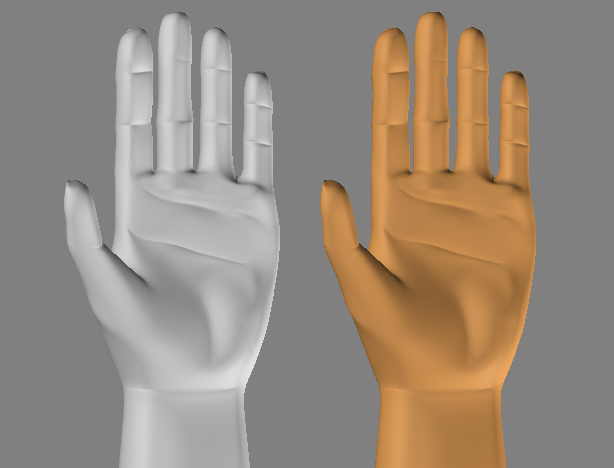
\includegraphics[width=0.5\textwidth]{Images/Blender.PNG}
    \caption{Virtual model of a prosthetic hand used with Interactive Myocontrol. The gray hand is used to reproduce the reference signals, whereas the orange hand is used to reproduce the predictions.}
    \label{fig:hand-blender}
\end{figure}
The hardware used to generate the sEMG signals from the muscular activation of human participants is the Myo Armband manufactured by Thalmic Labs (\href{https://www.thalmic.com}{https://www.thalmic.com}), is provided with eight sEMG sensors uniformly distributed along the bracelet.
\begin{figure}[ht]
    \centering
    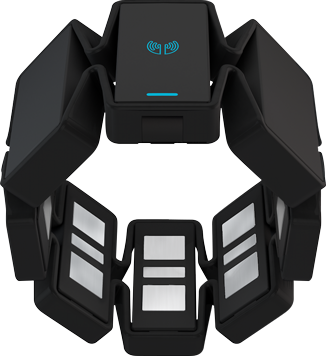
\includegraphics[width=0.5\textwidth]{Images/myo_armband.png}
    \caption{Myo Armband manufactured by \href{https://www.myo.com/techspecs}{Thalmic Labs}}
    \label{fig:myo_armband}
\end{figure}
The sEMG signals produced by the bracelet are the only input signal used by our machine learned controller, before being passed as input to the controller the signals are rectified and mildly low-pass filtered with a 2nd order Butterworth filter (cutoff 1Hz).
The outputs of the machine learned controller are nine different value which corresponds to the activation level of the nine different degrees of freedom (DOFs) of the prosthetic hand. In a real prosthetic hand these nine values are used to directly control the actuators which permits the movement of the hand, whereas in our case these values are used to control the position of the virtual model of the hand. Interactive Myocontrol use the different values of the nine DOFs to define 17 different action that are used as references in the training of the controller. In this work we are only interested in four of these actions, which are: rest, power grasp, wrist flexion and wrist extension; for convenience's sake we will consider as outputs the activation level of the above mentioned actions.
Interactive Myocontrol let the user decide which subset of the 17 actions desires to use in the training of the machine learned controller.
Therefore each sample of the training set $S$ is composed of an input sample $\mathbf{x}_i \in \mathbb{R}^8$ and a corresponding target value $\mathbf{y}_i \in \mathbb{R}^9$. In particular, given the physical limits of the sEMG sensors, each features of the input samples is limited between 0 and 5, therefore we can further limit the input space to $[0, 5]^8$.
As is customary in the current state of the art (see, eg., \cite{hahne2015concurrent}, \cite{sierra2013realistic}) in practice $S$ is built by gathering for each action of interest a certain number of observations while the participant is doing that particular action; each observation is then coupled with the target value associated to the action.
For example, the participant is asked to power grasp ("make a fist"); once the experimenter verifies that the signals have reached a stable pattern, well distinct from the baseline, a suitable number of observations is recorded and associated to (synthetic) target values denoting maximal activation of all fingers. This methodology is called on-off goal-directed training.
Interactive Myocontrol permits an incremental training of the machine learned controller: it is possible for the user to add new training samples after the initial training session and retrain the learning machine using also the new data; in \cite{Strazzulla2017} such machine learned controller is called \textit{Incremental-Learning Myoelectric Controller}
\section{dReal}\label{sec:dReal}
In this work we needed an SMT solver which could manage trascendent functions, due to the utilization of the Random Fourier Features as feature map in the machine learned controller. We chose dReal \cite{gao2013dreal} because it satisfied our requirements and was provided with an API python which could be easily used in our code. It was out of the scope of this thesis to compare the performance of different SMT solver, therefore we didn't consider others than dReal.
In order to handle a wide range of nonlinear real functions dReal implements the framework of $\delta$-complete decision procedures. We say a decision procedures is $\delta$-complete for a set of formulas $S$ if for any $\phi \in S$ the procedure returns \textit{unsat} if $\phi$ is unsatisfiable or \textit{$\delta$-sat} if $\phi^\delta$ is satisfiable.
$\delta$ is an arbitrary positive rational number and $\phi^\delta$ is a syntactic variant of $\phi$ that encodes a notion of numerical perturbation on logic formulas. Essentialy we relax the constrains on the procedure in order to permit answers with an one sided $\delta$-bounded error, therefore $\delta$-complete decision procedures can exploit the power of numerical approximations without losing formal correctness guarantees.
\chapter{Problem Definition}\label{ch:problem-definition}
\section{Introduction}\label{sec:pd-intro}
The system we consider in this thesis is Interactive Myocontrol (section \ref{sec:interactivemyocontrol}), as we have seen in the relative section the input data of our machine learned controller comes from the eight sEMG sensors of the myobracelet and the output data are the activation levels of the nine DOFs of the prosthetic hand.
The problem we are going to study is what we call \textit{activation overshooting}: whenever a participant increase her muscle activation we expect that the prosthesis would in turn increase the applied force / torque; however, if we have a non-linear learning model like the one used in Interactive Myocontrol, this behaviour is not guaranteed. This kind of behaviour should be prevented and avoided by all means because can easily lead to potentially catastrophic failures: in practice whenever a participants increase her force in order to acquire, for example, a better grip on an object the results is the opposite to her expectation, e.g. the prosthesis drop the object.
Overshooting cannot be easily solved gathering more training data for the participant: this would require her to apply a large amount of force which could lead her to muscle strain, fatigue and frustration. Therefore we decided to study in the direction of "mechanically" amend the machine learning model in order to make it more reliable with respect to overshooting.
%
%
%
\section{Formal Definition}\label{sec:pd-formal-def}
In order to be able to amend the machine using an automated procedure we needed to define the overshooting problem in a strictly formal way: in the following we show how we arrived to the formal definition.
For sake of convenience we briefly consider a 2D-reduced exemplary S in which are contained the samples generated by three actions: rest, power grasp and wrist flexion. As can be seen in figure \ref{fig:heatmap} the training set can be seen as a set of clusters, each corresponding to a certain action.
\begin{figure}[ht]
    \centering
    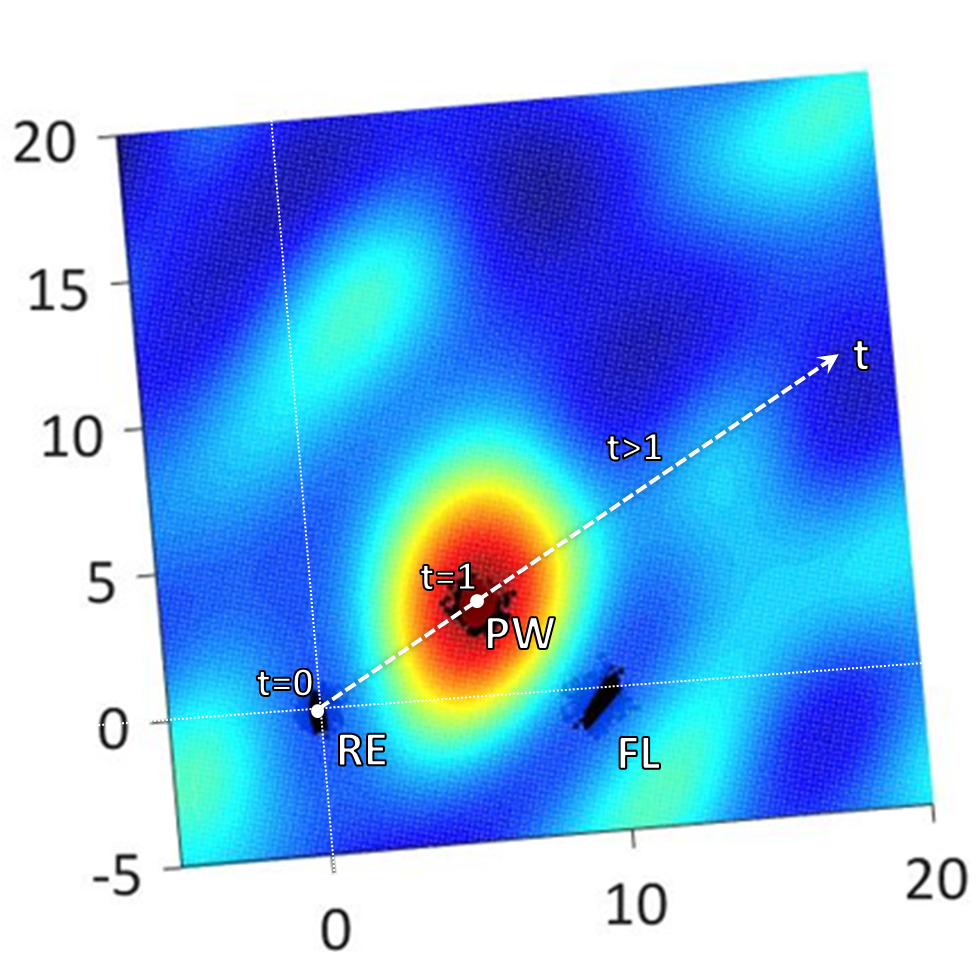
\includegraphics[width=0.8\textwidth]{Images/heatmap_DOF1.png}
    \caption{A 2D-reduced exemplary dataset S, obtained after gathering observations for three actions (black dots; rest, RE; power grasp, PW; wrist flexion, FL); the colour of the heat map denotes the value of the target value for power grasping, $f_{PW}$ . Values of the input space lying on the straight line $\overline{RE} + (\overline{PW} - \overline{RE})t_{PW}$ roughly denote power grasping with increasing strength.}
    \label{fig:heatmap}
\end{figure}
We define as $\overline{RE}$, $\overline{PW}$, $\overline{FL}$ the centers of the clusters corresponding respectively to the actions rest, power grasp and wrist flexion. In the figure is possible to see, as an heatmap, the function $f_{PW}$ obtained by training the learning model seen in section \ref{sec:ML} using the training set S.  
We decided to assume the straight line of the type $\overline{RE} + (\overline{PW} - \overline{RE})t_{PW}$ as the zone of the input space along which the participants signals move when she increase or decrease the force applied to a certain action; this assumption is justified by the physiology of the muscular activation and by our experimental observation.
As can be seen in figure \ref{fig:heatmap} between $t_{PW} = 0$ and $t_{PW} = 1$ the behaviour of the model is what we expected: the value of $f_{PW}$ increase with $t_{PW}$ and assume the maximum value for $t_{PW} = 1$, which corresponds to $\overline{PW}$. The problem become clear for the values of $t_{PW}$ greater than 1: almost immediately $f_{PW}$ begin to decrease and reaches 0 for $t_{PW} \approx 2$. In practice, the participant tries to apply more force and instead the hand open up, leading to drop the grasped object. This kind of failure is what we have called overshooting.
We are now able to give a formal definition of a model subject to overshooting:
\begin{equation}
    \exists A,t_A>1 : x = \overline{RE} + (\overline{A} - \overline{RE})t_{A} \implies f_A(x) < A_{max}
    \label{eq:overshooting}
\end{equation}
where $A$ indicates a general action on which we have trained the model and $A_{max}$ is the maximum activation value for that action. The other quantities correspond to what we have seen before but for a general action $A$.
Obviously the muscular activation in reality is not as precise and constant as we have supposed, therefore it will deviates from the straight line $\overline{RE} + (\overline{A} - \overline{RE})t_{A}$ and, as consequence, our definition of model subject to overshooting doesn't represent all the possible instances of overshooting. Nonetheless, thanks to the continuity of the nonlinear model we have chosen (RR-RFF sec. \ref{sec:ML}), the automated mending process manages to overall enhance the reliability of the system with respect to overshooting.
Overshooting can probably be defined in other ways, nevertheless we prefer to stick with the definition given in equation \ref{eq:overshooting} in order to limit as much as possible the subset of the input space we need to analyse to guarantee the absence of overshooting.
%
%
%
\section{Automated Procedure}
After having formally defined the overshooting problem we studied how to design an automated procedures which could bring the model to a state in which it wasn't subject to our definition of overshooting. In order to do so without changing drastically the structure of the learning model and of Interactive Myocontrol we decided to follow in the step of \cite{Strazzulla2017} and leverage the incrementality of the learning model used by Interactive Myocontrol.
The general idea of our automated procedure is to generate synthetic labelled samples which are then added to the original training set in order to modify the model and bring it in a state in which it is not subject to overshooting. With equation \ref{eq:overshooting} we have already given a preliminary definition of point in the input space which are affected by overshooting, it is reasonable to consider the above mentioned points as the one we are interested to add to the training set in order to modify the model so that they present the correct labels (e.g. they are no more subject to overshooting).
In order to preserve the coherence of the learning method we decided to keep the way we add points to the training set as similar as possible to the way the original training points are gathered: as seen before the training data are distributed in clusters corresponding to the different actions, therefore also our synthetic data will be distributed in the same way.
Given the characteristic of the training model and the possible interaction between the different actions, we decided to design our automated repair procedure as a iterative one:
\begin{enumerate}
    \item For each action of interest we search for an unsafe point (e.g. a point subject to overshooting, see equation \ref{eq:overshooting}), if no unsafe point is found for every action then the repair process is completed successfully.
    \item For each action for which we have found an unsafe point we generate a cluster centred on the point and we associate each point of the cluster with an appropriate label, then we add the point generated to the training set. We do nothing for the action for which we haven't found an unsafe point.
    \item The learning model is trained again but this time on the modified training set, then we continue with point 1.
\end{enumerate}
Obviously we still need to decide how to determine the appropriate label for the points we add to the training set: the natural choice appears to be the value $A_{max}$ seen in equation \ref{eq:overshooting} but experimentally we have found out that this kind of choice brings the repair procedure to need a longer time, and more unsafe points, in order to completely repair the model. This result is quite easy to understand: if our \textit{unsafety} condition is defined by equations \ref{eq:overshooting} we want that to every points $x = \overline{RE} + (\overline{A} - \overline{RE})t_{A}$ with $t_{A} >= 1$ corresponds a target value $f_A(x) >= A_{max}$ and if we consider the continuity of the learning model we have chosen, the adding of points with synthetic target value equals to $A_{max}$ it's unlikely to drastically modify the original model. Moreover from a theoretical point of view we would expect that to greater values of the input signals would correspond a greater activation level of the action. Therefore we chose as activation level for each synthetic point $x$ a value given by the following equation:
\begin{equation}
    y_{syn} = y_0 + c_A \cdot (x_{proj} - \overline{RE})
    \label{eq:output_unsafe}
\end{equation}
where $c_A$ is the slope of the straight line connecting $(\overline{RE}, 0)$ and $(\overline{A}, A_{max})$ in the space $\mathbb{R}^9$ (e.g. remember that the input space is $\mathbb{R}^8$ and the activation value is a real number), $x_{proj}$ is the projection of the point $x$ on the straight line $\overline{RE} + (\overline{A} - \overline{RE})t_{A}$ and $y_0$ is a quantity we have determined experimentally.
For what concern the generation of the clusters we have chosen to draw the points from a normal distribution with mean equals to the original unsafe point and variance equals to the variance of the cluster generated during the training corresponding to the action of interest. The number of points drawn is equal to the number of point of the original cluster.
The last problem we need to solve before being able to implement our automated repair process is how we can find the unsafe points: in this thesis we have studied two different methods to do so.
The first method we have considered use an SMT solver in order to search for unsafe points: the problem is encoded as a propositional logic formula and then the SMT solver is used to find a solution of such formula, in equation \ref{eq:SMT-formula} we show the logic formula we give to the SMT solver.
\begin{equation}
\begin{aligned}
    t \geq t_{min} \wedge t \leq t_{max}\qquad \wedge \\
    \mathbf{\phi}(t) = cos(\sigma \cdot \mathbf{\Omega} \cdot (\overline{RE} + (\overline{A} - \overline{RE})t)\qquad \wedge \\
    y = \mathbf{w}^T \phi(t)\qquad \wedge \\
    y < A_{max}\qquad\quad
    \label{eq:SMT-formula}
\end{aligned}
\end{equation}
where $t_{min}$ and $t_{max}$ define the interval of the straight line we are interested in and the other quantities are the same we have defined in the previous sections. The main difference from the learning model seen in section \ref{sec:ML} is that we have $\phi(t)$ instead of $\phi(\mathbf{x})$: actually there is no real difference, we have only highlighted the dependence from the variable t. Changing the dependence from $\mathbf{x}$ to only $t$ radically simplify the work of the SMT solver: the space it needs to analyse goes from $\mathbb{R}^8$ to just $\mathbb{R}$. This simplification is what make possible to use an SMT solver: in the preliminary test we have done, using a formulation of the problem which used $\mathbf{x}$ instead of $t$ as variable, the solver wasn't able to complete successfully the analysis due to the excessive computational complexity. We have called SMT-repair the repair process which uses this method to find the unsafe points.\\
The second method we have considered consists in generating a set of point uniformly distributed along the straight line corresponding to the action of interest, computing their target values and analysing them in order to find one that doesn't respect the safety condition. In this case we are able to search for \textit{the unsafest} point, e.g. the point $\mathbf{x}$ which maximise the quantity $A_{max} - f(\mathbf{x})$. We have called PDO-Repair the repair process which uses this method to find the unsafe points.\\
At this point we have managed to design all the parts of the automated procedure, therefore we just need to put them together. Below we show a pseudocode of our procedure:
\vspace{5mm}\small
\begin{algorithmic}
	\STATE $\mathbf{w} \gets \mathbf{buildModel}(S)$
	\STATE $unsafe \gets True$
	\WHILE{$unsafe$}
	\FOR{\textbf{each action} $A$}
	\STATE [$unsafe$ ,$t_A^U$] $\gets \mathbf{safetyCheck}(\mathbf{w}, S)$
	\IF{$unsafe$}
	\STATE $(X',Y') \gets (\mathcal{N}(t_A^U,\sigma_A),\mathbf{y}_A)$
	\STATE $\mathbf{w} \gets \mathbf{buildModel}(S \cup (X',Y'))$
	\ENDIF
	\ENDFOR
	\ENDWHILE
\end{algorithmic}
\vspace{5mm}\normalsize
In the pseudocode above the function $\mathbf{safetyCheck}(...)$ represent one of the two methods we have considered in this section and $\mathbf{buildModel}(...)$ represent the training of the learning model. In the following we show how the model change during the execution of the repair procedure for both the safety check methods.
\subsection{Execution of PDO-Repair}\label{subsec:PDO-Repair}
The following images show an example of an execution of the PDO-Repair on a training set which consider the actions: power grasp, wrist flexion and wrist extension. In particular we show the progress of the model along the straight lines we have considered during this section.
\begin{figure}[ht]
    \centering
    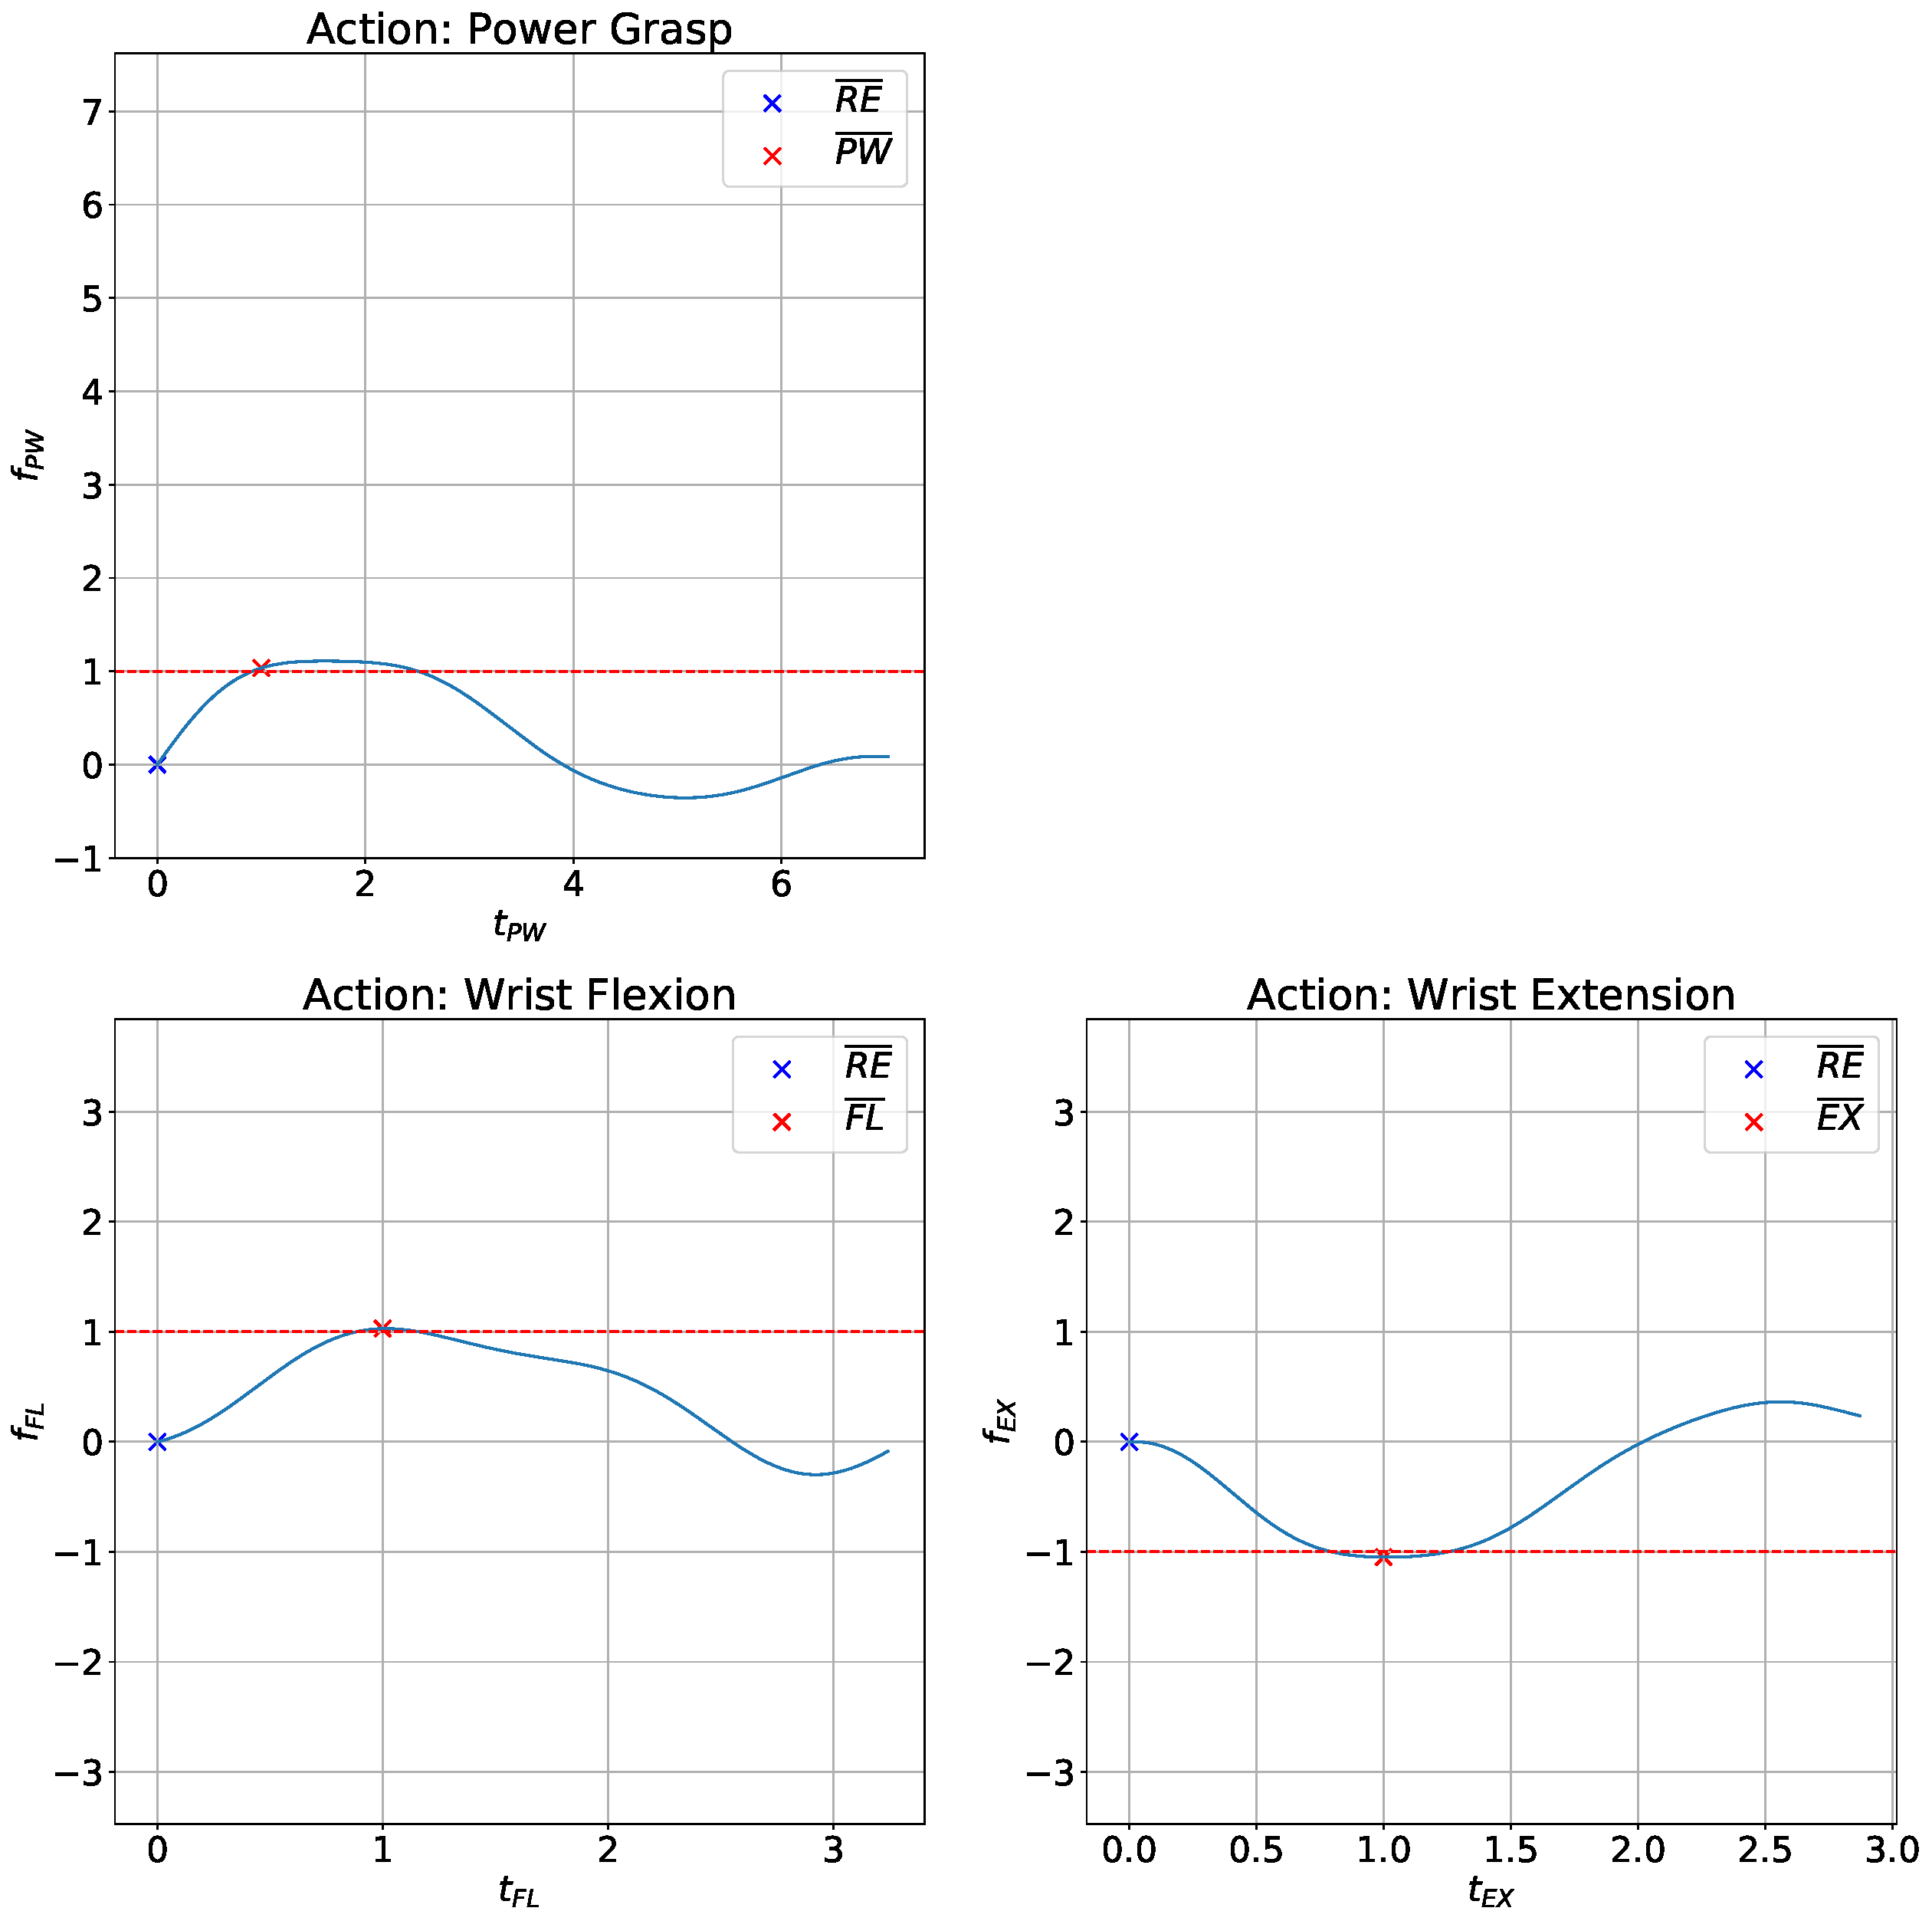
\includegraphics[width=\textwidth]{Images/repair-example/PDO-State0.pdf}
    \caption{In this figure we show the original model along the straight lines $\overline{RE} + (\overline{PW} - \overline{RE})t_{PW}$, $\overline{RE} + (\overline{FL} - \overline{RE})t_{FL}$ and $\overline{RE} + (\overline{EX} - \overline{RE})t_{EX}$. As can be seen the model is subject to overshooting along all the three lines. The red dashed lines represent the maximum activation values for the different actions.}
    \label{fig:PDO-exec-0}
\end{figure}
It can be noted in figure \ref{fig:PDO-exec-0} that for the action $EX$ the target value is negative (to be precise $EX_{max} = 1$), this fact doesn't change what we have seen till now: the extension of the automated procedure to this case is trivial. The negative target value is due to the fact that $FL$ and $EX$ correspond to the same degree of freedom, therefore they present opposite activation value. The belonging to the same degree of freedom of the two actions is easily understood considering that they are physically mutually exclusive, e.g. it is impossible to flex and extend the wrist at the same time. Moreover, as far as we know, in all the prosthetic hand the two action are managed by the same actuator.
\begin{figure}[ht]
    \centering
    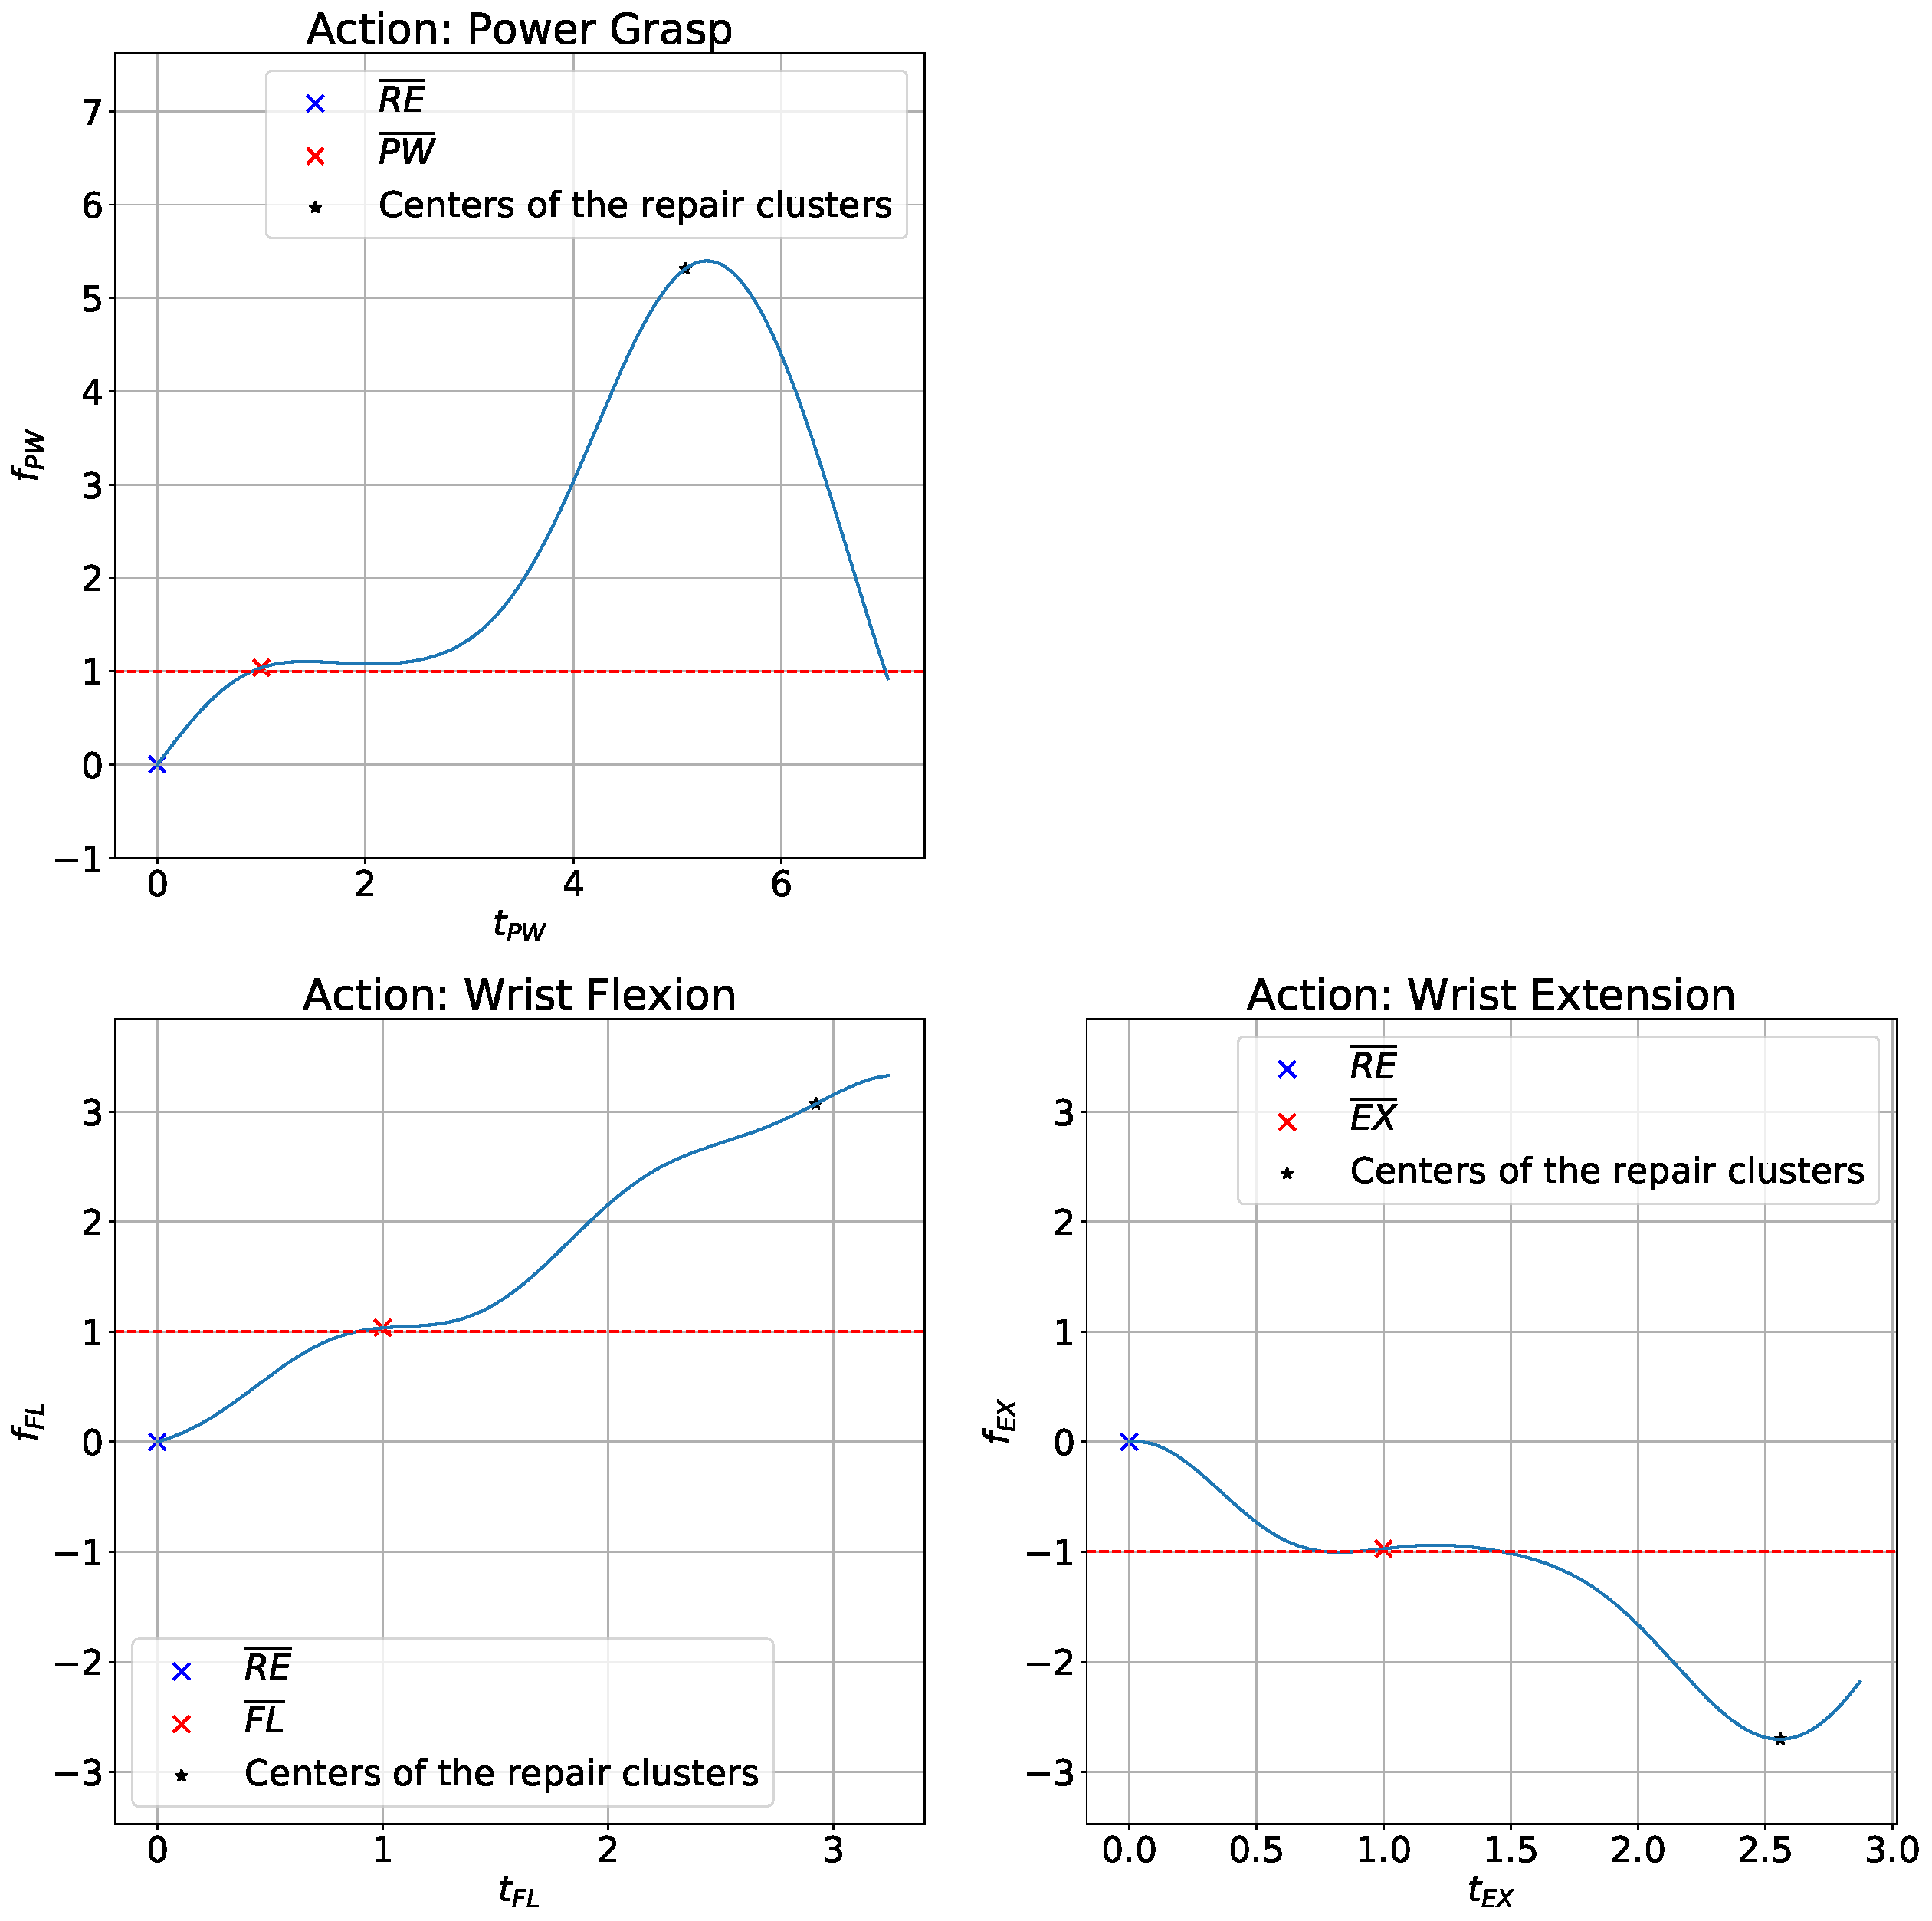
\includegraphics[width=\textwidth]{Images/repair-example/PDO-State1.pdf}
    \caption{In this figure we show the model along the straight lines $\overline{RE} + (\overline{PW} - \overline{RE})t_{PW}$, $\overline{RE} + (\overline{FL} - \overline{RE})t_{FL}$ and $\overline{RE} + (\overline{EX} - \overline{RE})t_{EX}$ after the first round of repair. The red dashed lines represent the maximum activation values for the different actions.}
    \label{fig:PDO-exec-1}
\end{figure}
Comparing figures \ref{fig:PDO-exec-1} and \ref{fig:PDO-exec-2} permits to see that the repair of the model along the straight lines is done only when it is needed: between the first and second iteration of the repair process there is no repair done along the straight line of the action $FL$, whereas the repair proceeds for the other two lines.
\begin{figure}[ht]
    \centering
    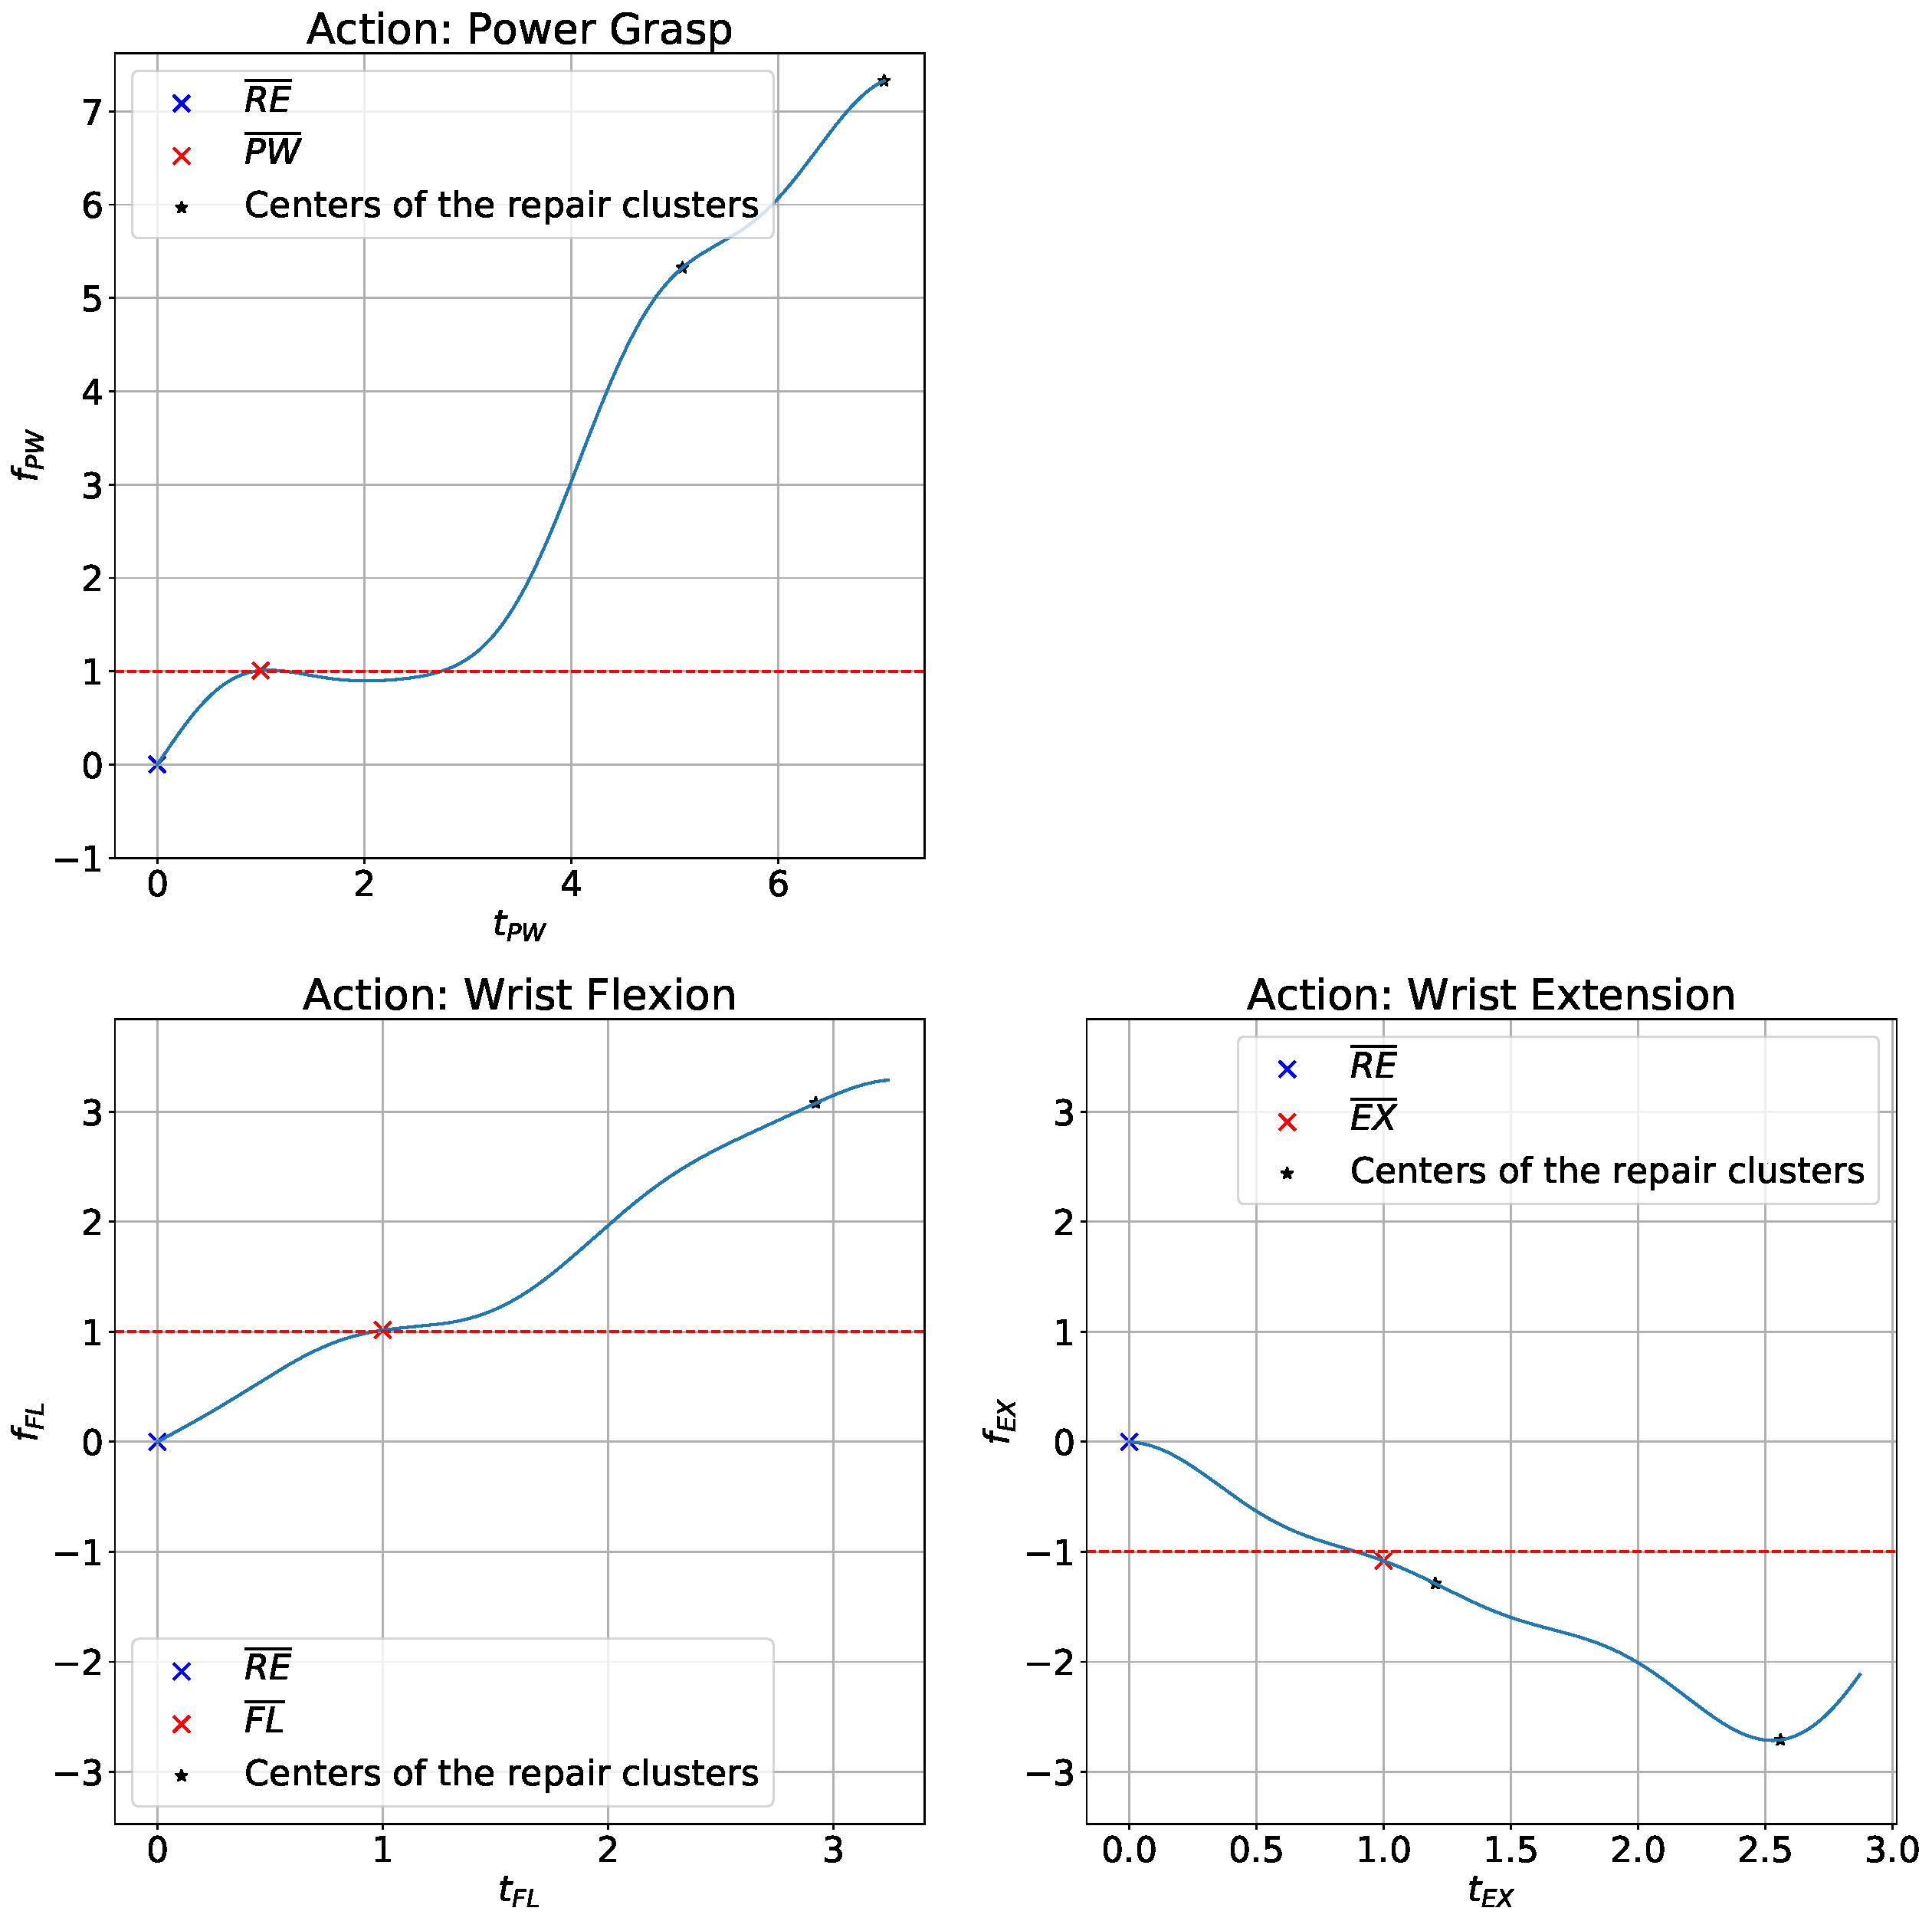
\includegraphics[width=\textwidth]{Images/repair-example/PDO-State2.pdf}
    \caption{In this figure we show the model along the straight lines $\overline{RE} + (\overline{PW} - \overline{RE})t_{PW}$, $\overline{RE} + (\overline{FL} - \overline{RE})t_{FL}$ and $\overline{RE} + (\overline{EX} - \overline{RE})t_{EX}$ after the second round of repair. The red dashed lines represent the maximum activation values for the different actions.}
    \label{fig:PDO-exec-2}
\end{figure}
It is also possible to see that, due to the characteristic of the learning model, the repair done in a particular point can bring to the appearance of unsafety in other points, therefore the necessity of an iterative repair procedure.
\begin{figure}[H]
    \centering
    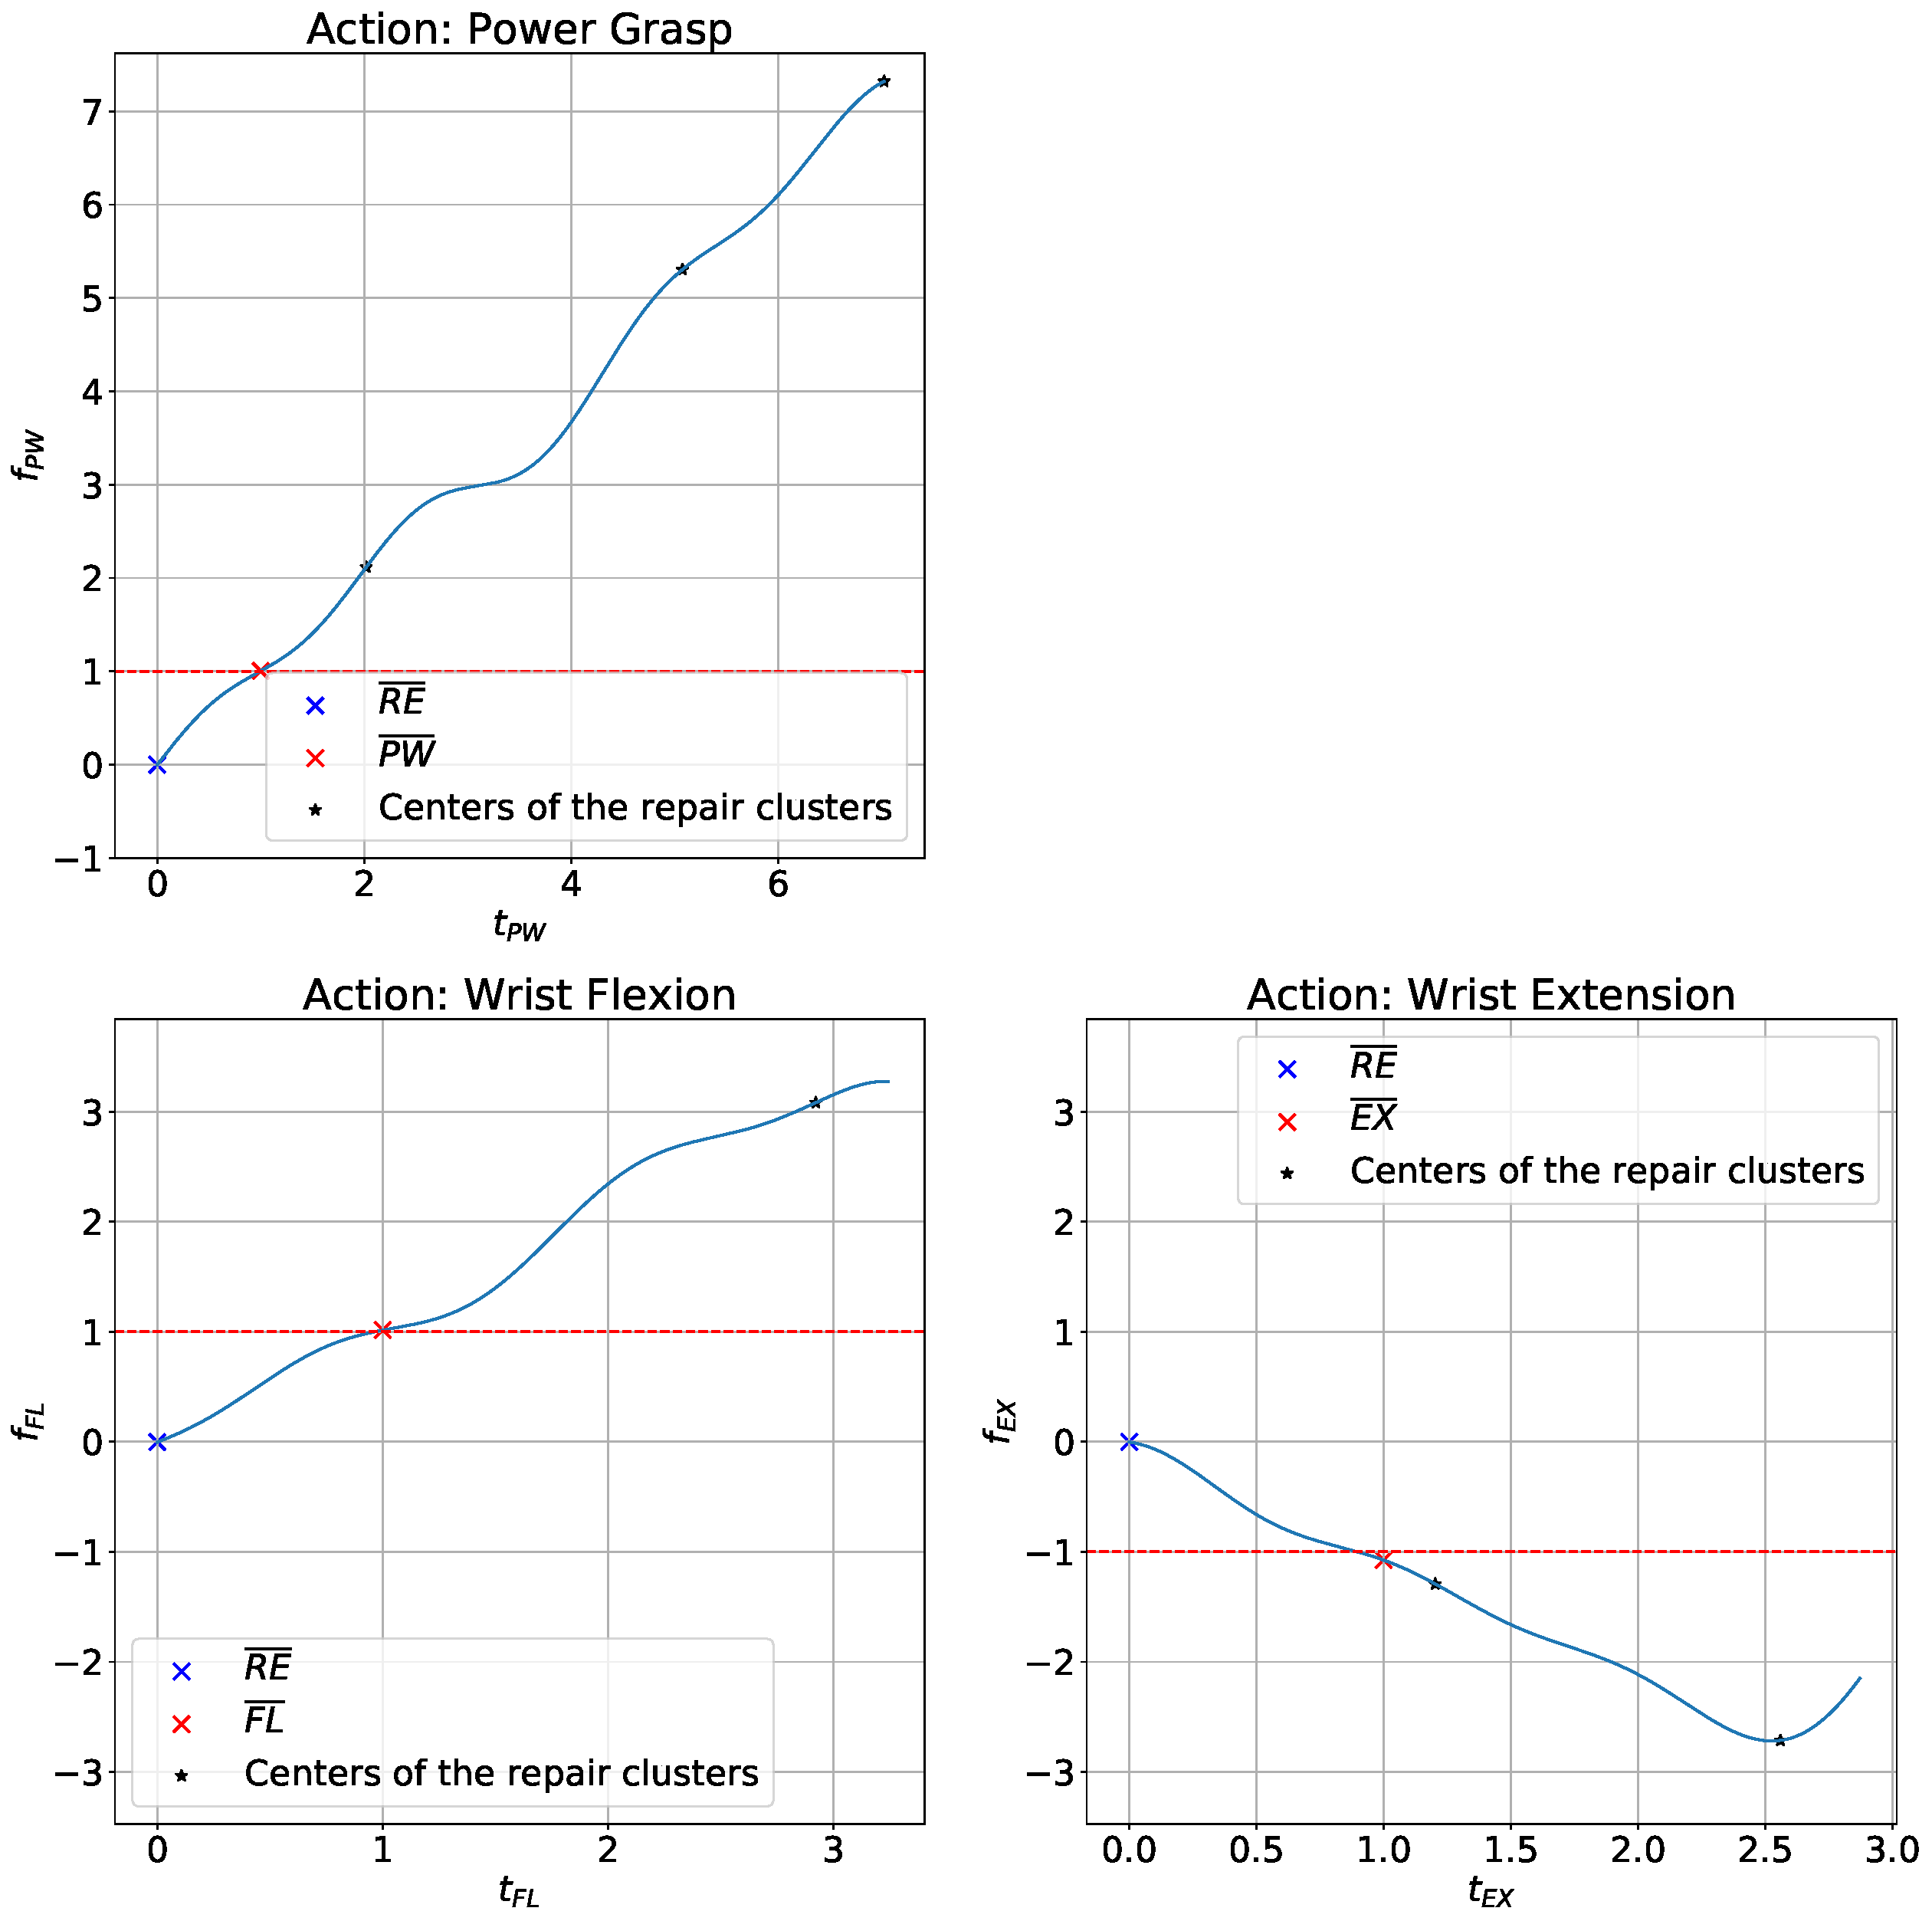
\includegraphics[width=\textwidth]{Images/repair-example/PDO-State3.pdf}
    \caption{In this figure we show the model along the straight lines $\overline{RE} + (\overline{PW} - \overline{RE})t_{PW}$, $\overline{RE} + (\overline{FL} - \overline{RE})t_{FL}$ and $\overline{RE} + (\overline{EX} - \overline{RE})t_{EX}$ after the final round of repair. The red dashed lines represent the maximum activation values for the different actions.}
    \label{fig:PDO-exec-3}
\end{figure}
As can be seen in figure \ref{fig:PDO-exec-3} the result of the repair process it is similar to a linearization of the functions $f_{PW}$, $f_{FL}$ and $f_{EX}$, which is quite reasonable: in general we would expect that to a linear increase in the muscular force applied would correspond a linear increase in the activation of a certain action.
%
%
\subsection{Execution of SMT-Repair}\label{subsec:SMT-Repair}
The following images show an example of an execution of the SMT-Repair on the same training set used for the example of the PDO-Repair.
\begin{figure}[H]
    \centering
    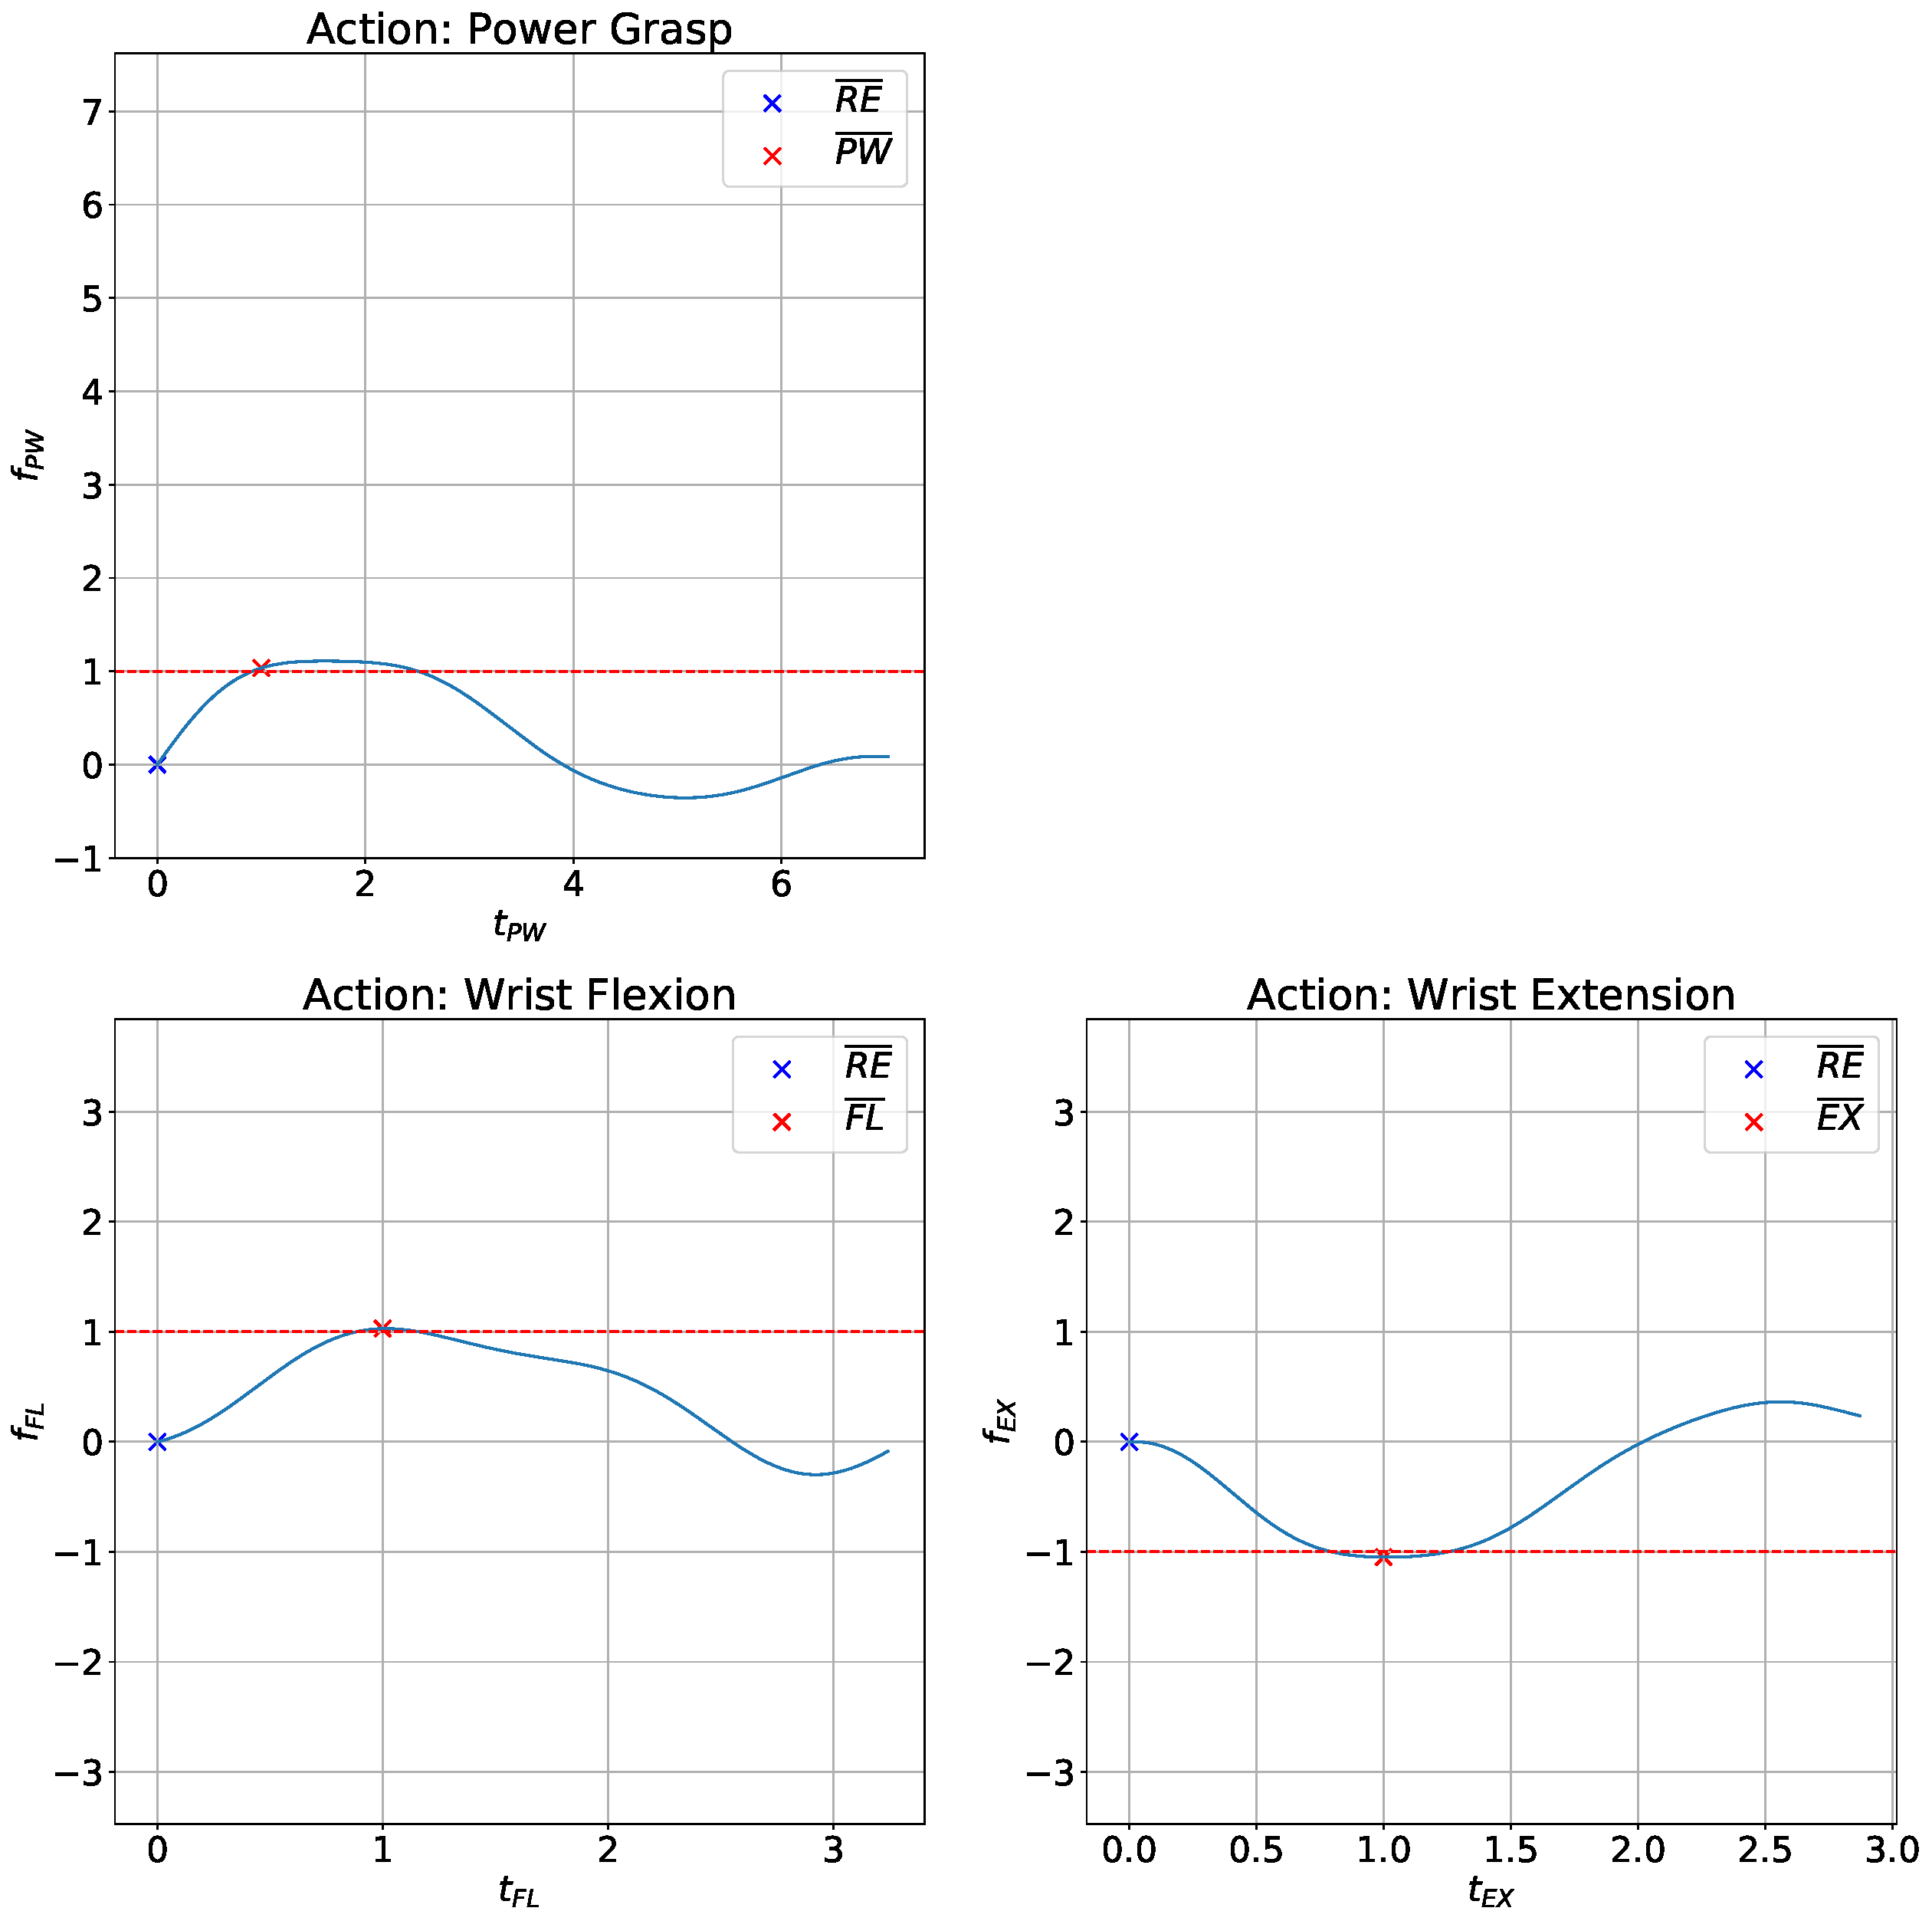
\includegraphics[width=\textwidth]{Images/repair-example/SMT-State0.pdf}
    \caption{In this figure we show the original model along the straight lines $\overline{RE} + (\overline{PW} - \overline{RE})t_{PW}$, $\overline{RE} + (\overline{FL} - \overline{RE})t_{FL}$ and $\overline{RE} + (\overline{EX} - \overline{RE})t_{EX}$. The red dashed lines represent the maximum activation values for the different actions.}
    \label{fig:SMT-exec-0}
\end{figure}
\begin{figure}[H]
    \centering
    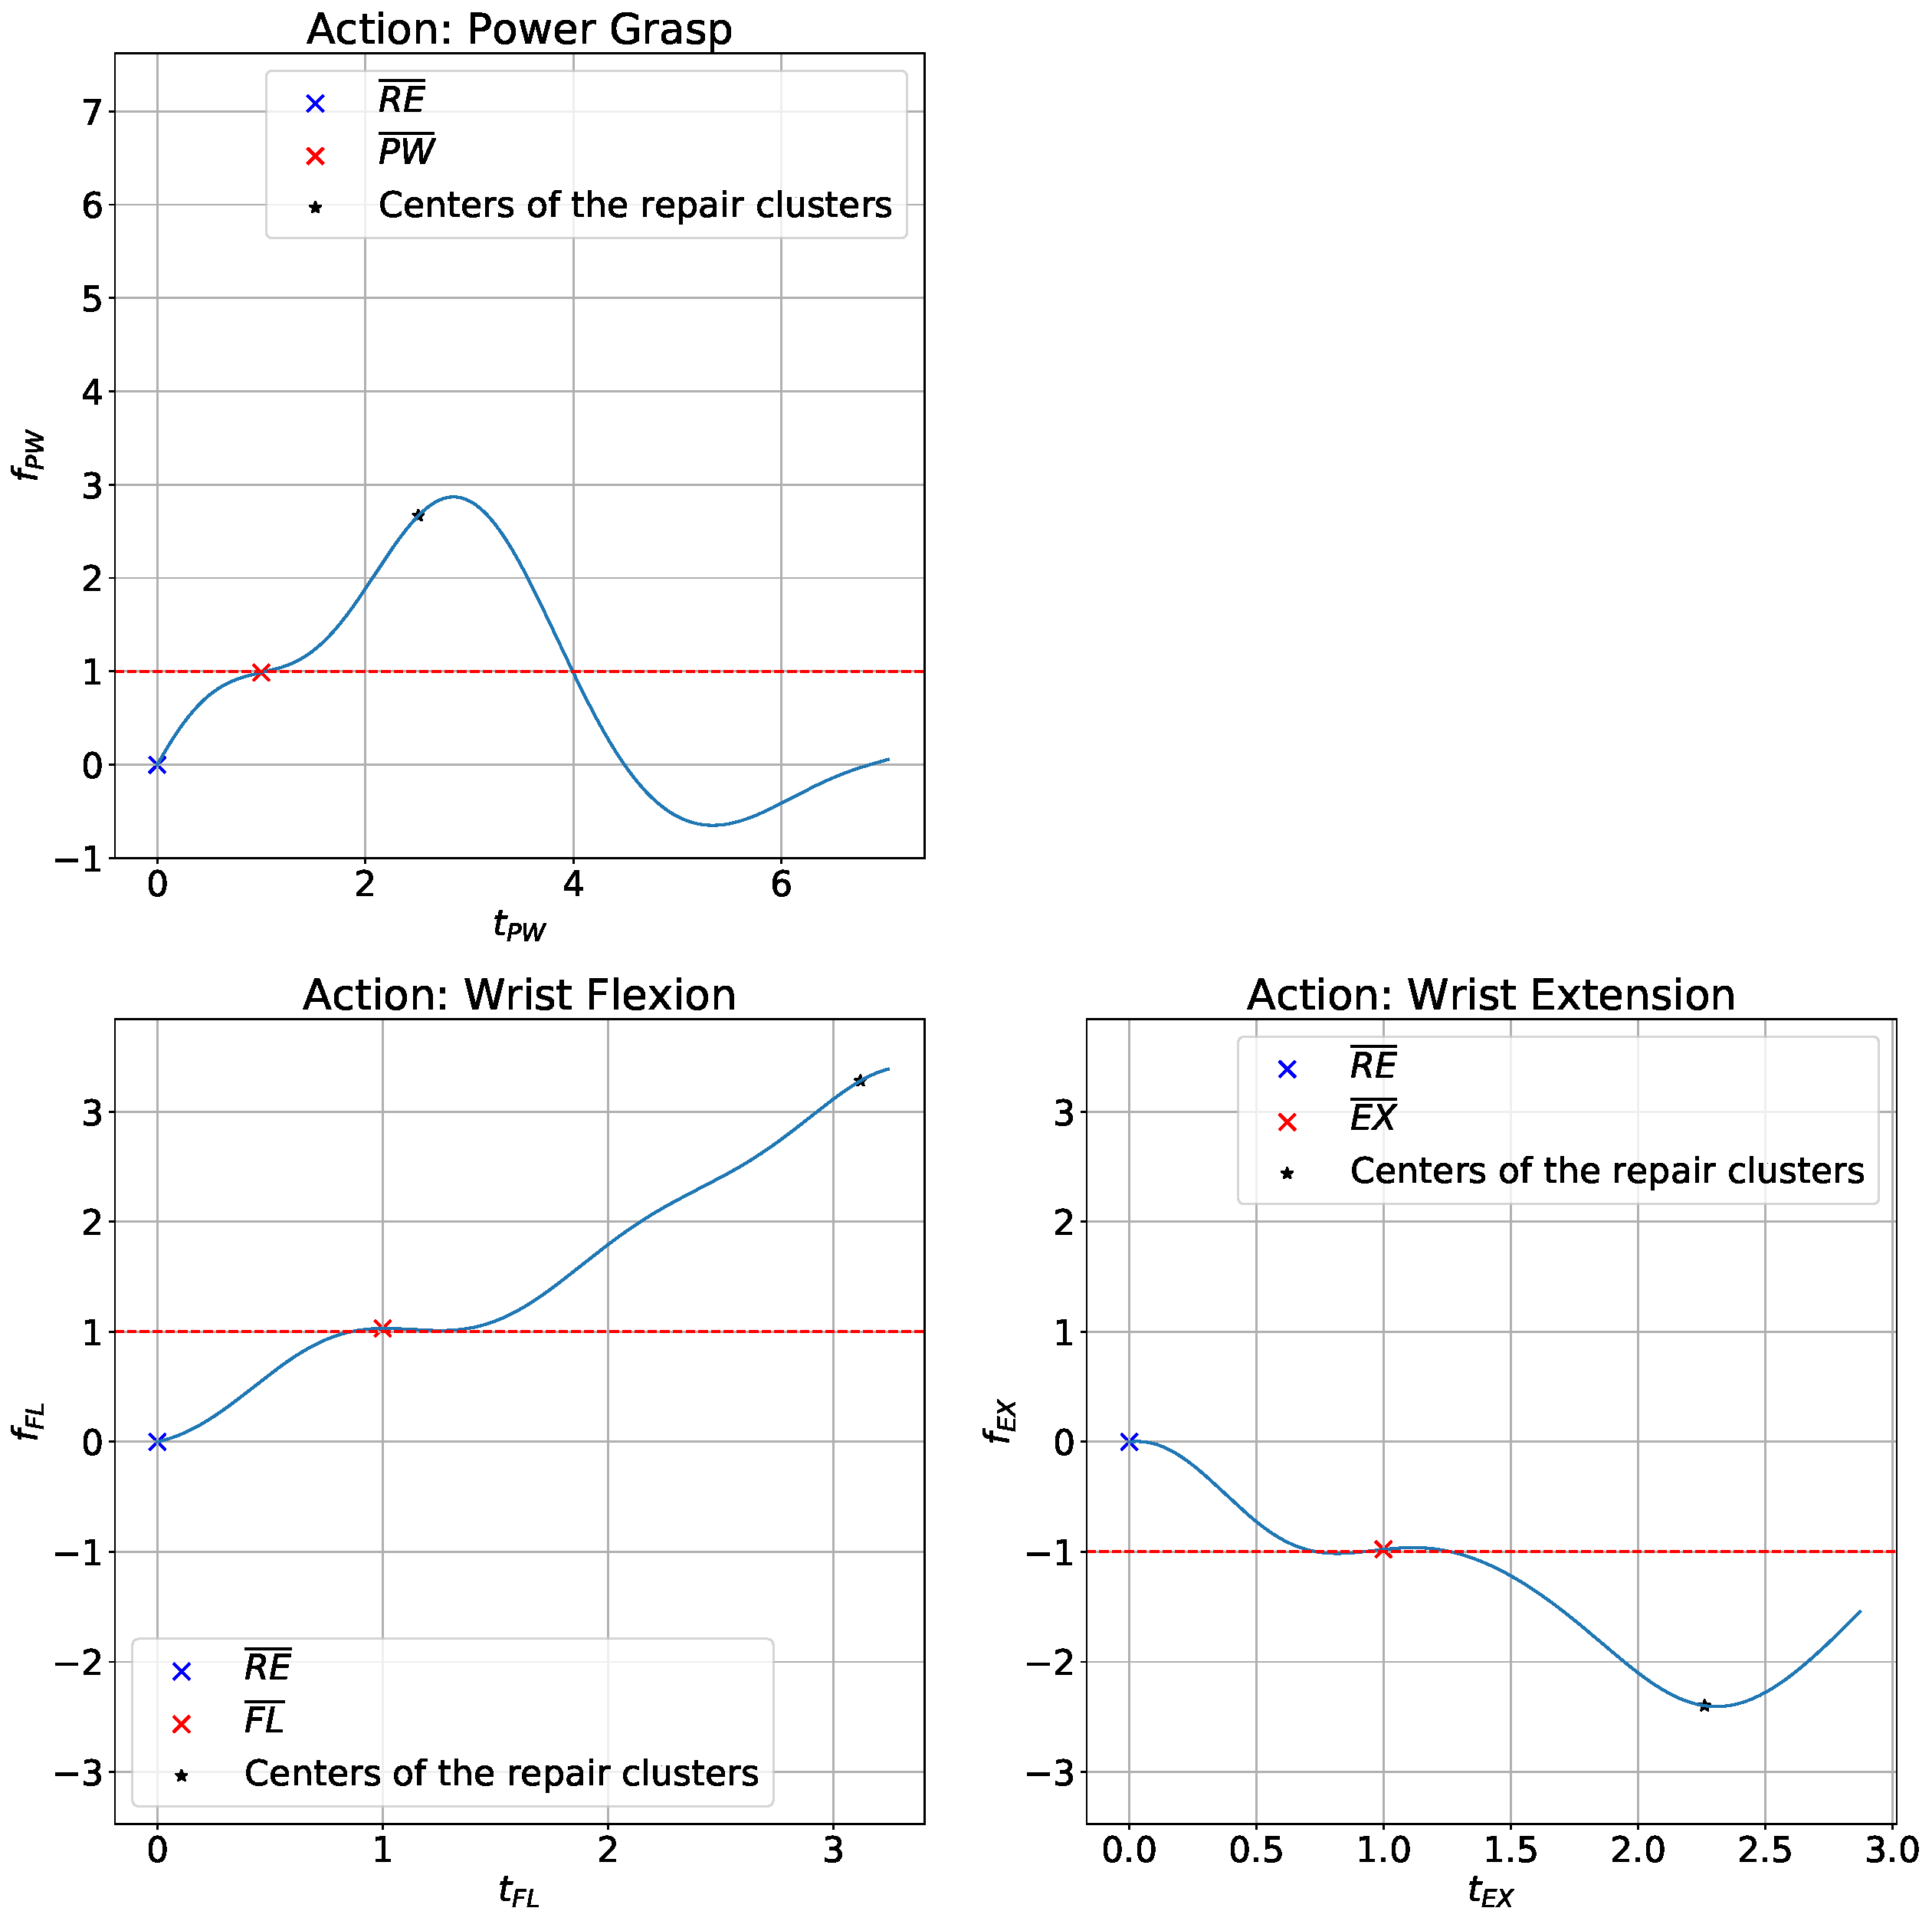
\includegraphics[width=\textwidth]{Images/repair-example/SMT-State1.pdf}
    \caption{In this figure we show the model along the straight lines $\overline{RE} + (\overline{PW} - \overline{RE})t_{PW}$, $\overline{RE} + (\overline{FL} - \overline{RE})t_{FL}$ and $\overline{RE} + (\overline{EX} - \overline{RE})t_{EX}$ after the first round of repair. The red dashed lines represent the maximum activation values for the different actions.}
    \label{fig:SMT-exec-1}
\end{figure}
\begin{figure}[H]
    \centering
    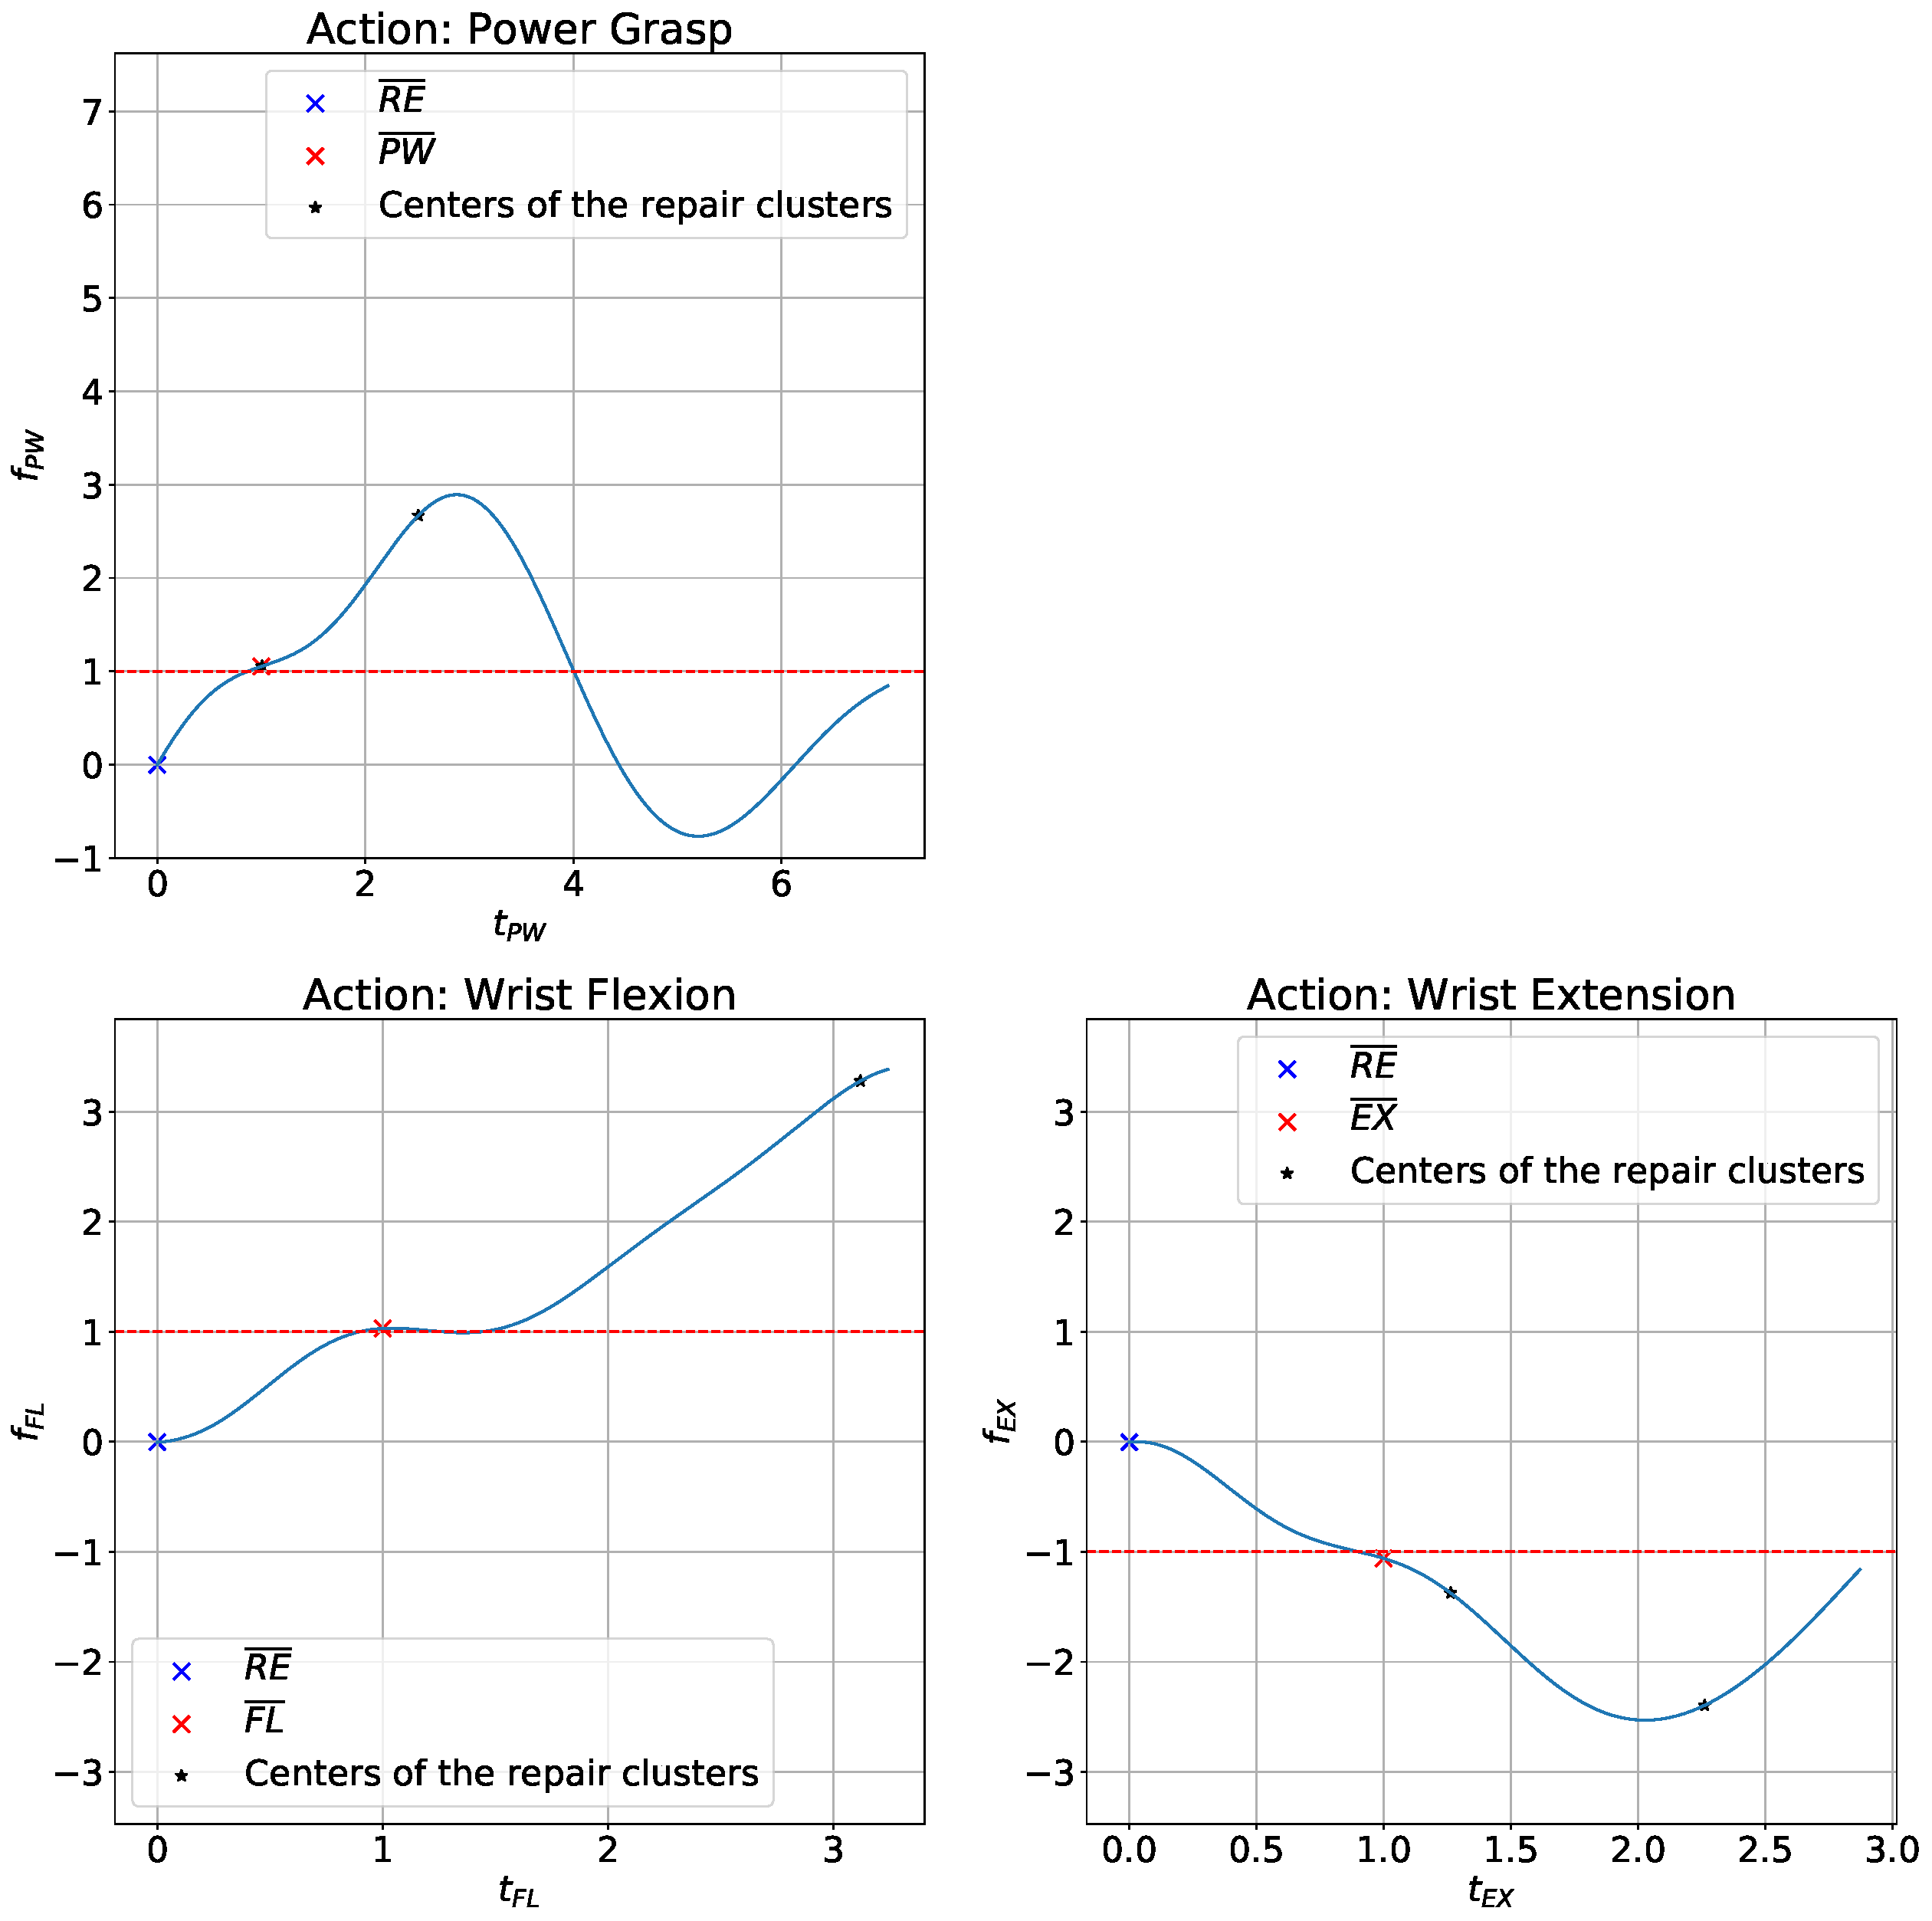
\includegraphics[width=\textwidth]{Images/repair-example/SMT-State2.pdf}
    \caption{In this figure we show the model along the straight lines $\overline{RE} + (\overline{PW} - \overline{RE})t_{PW}$, $\overline{RE} + (\overline{FL} - \overline{RE})t_{FL}$ and $\overline{RE} + (\overline{EX} - \overline{RE})t_{EX}$ after the second round of repair. The red dashed lines represent the maximum activation values for the different actions.}
    \label{fig:SMT-exec-2}
\end{figure}
\begin{figure}[H]
    \centering
    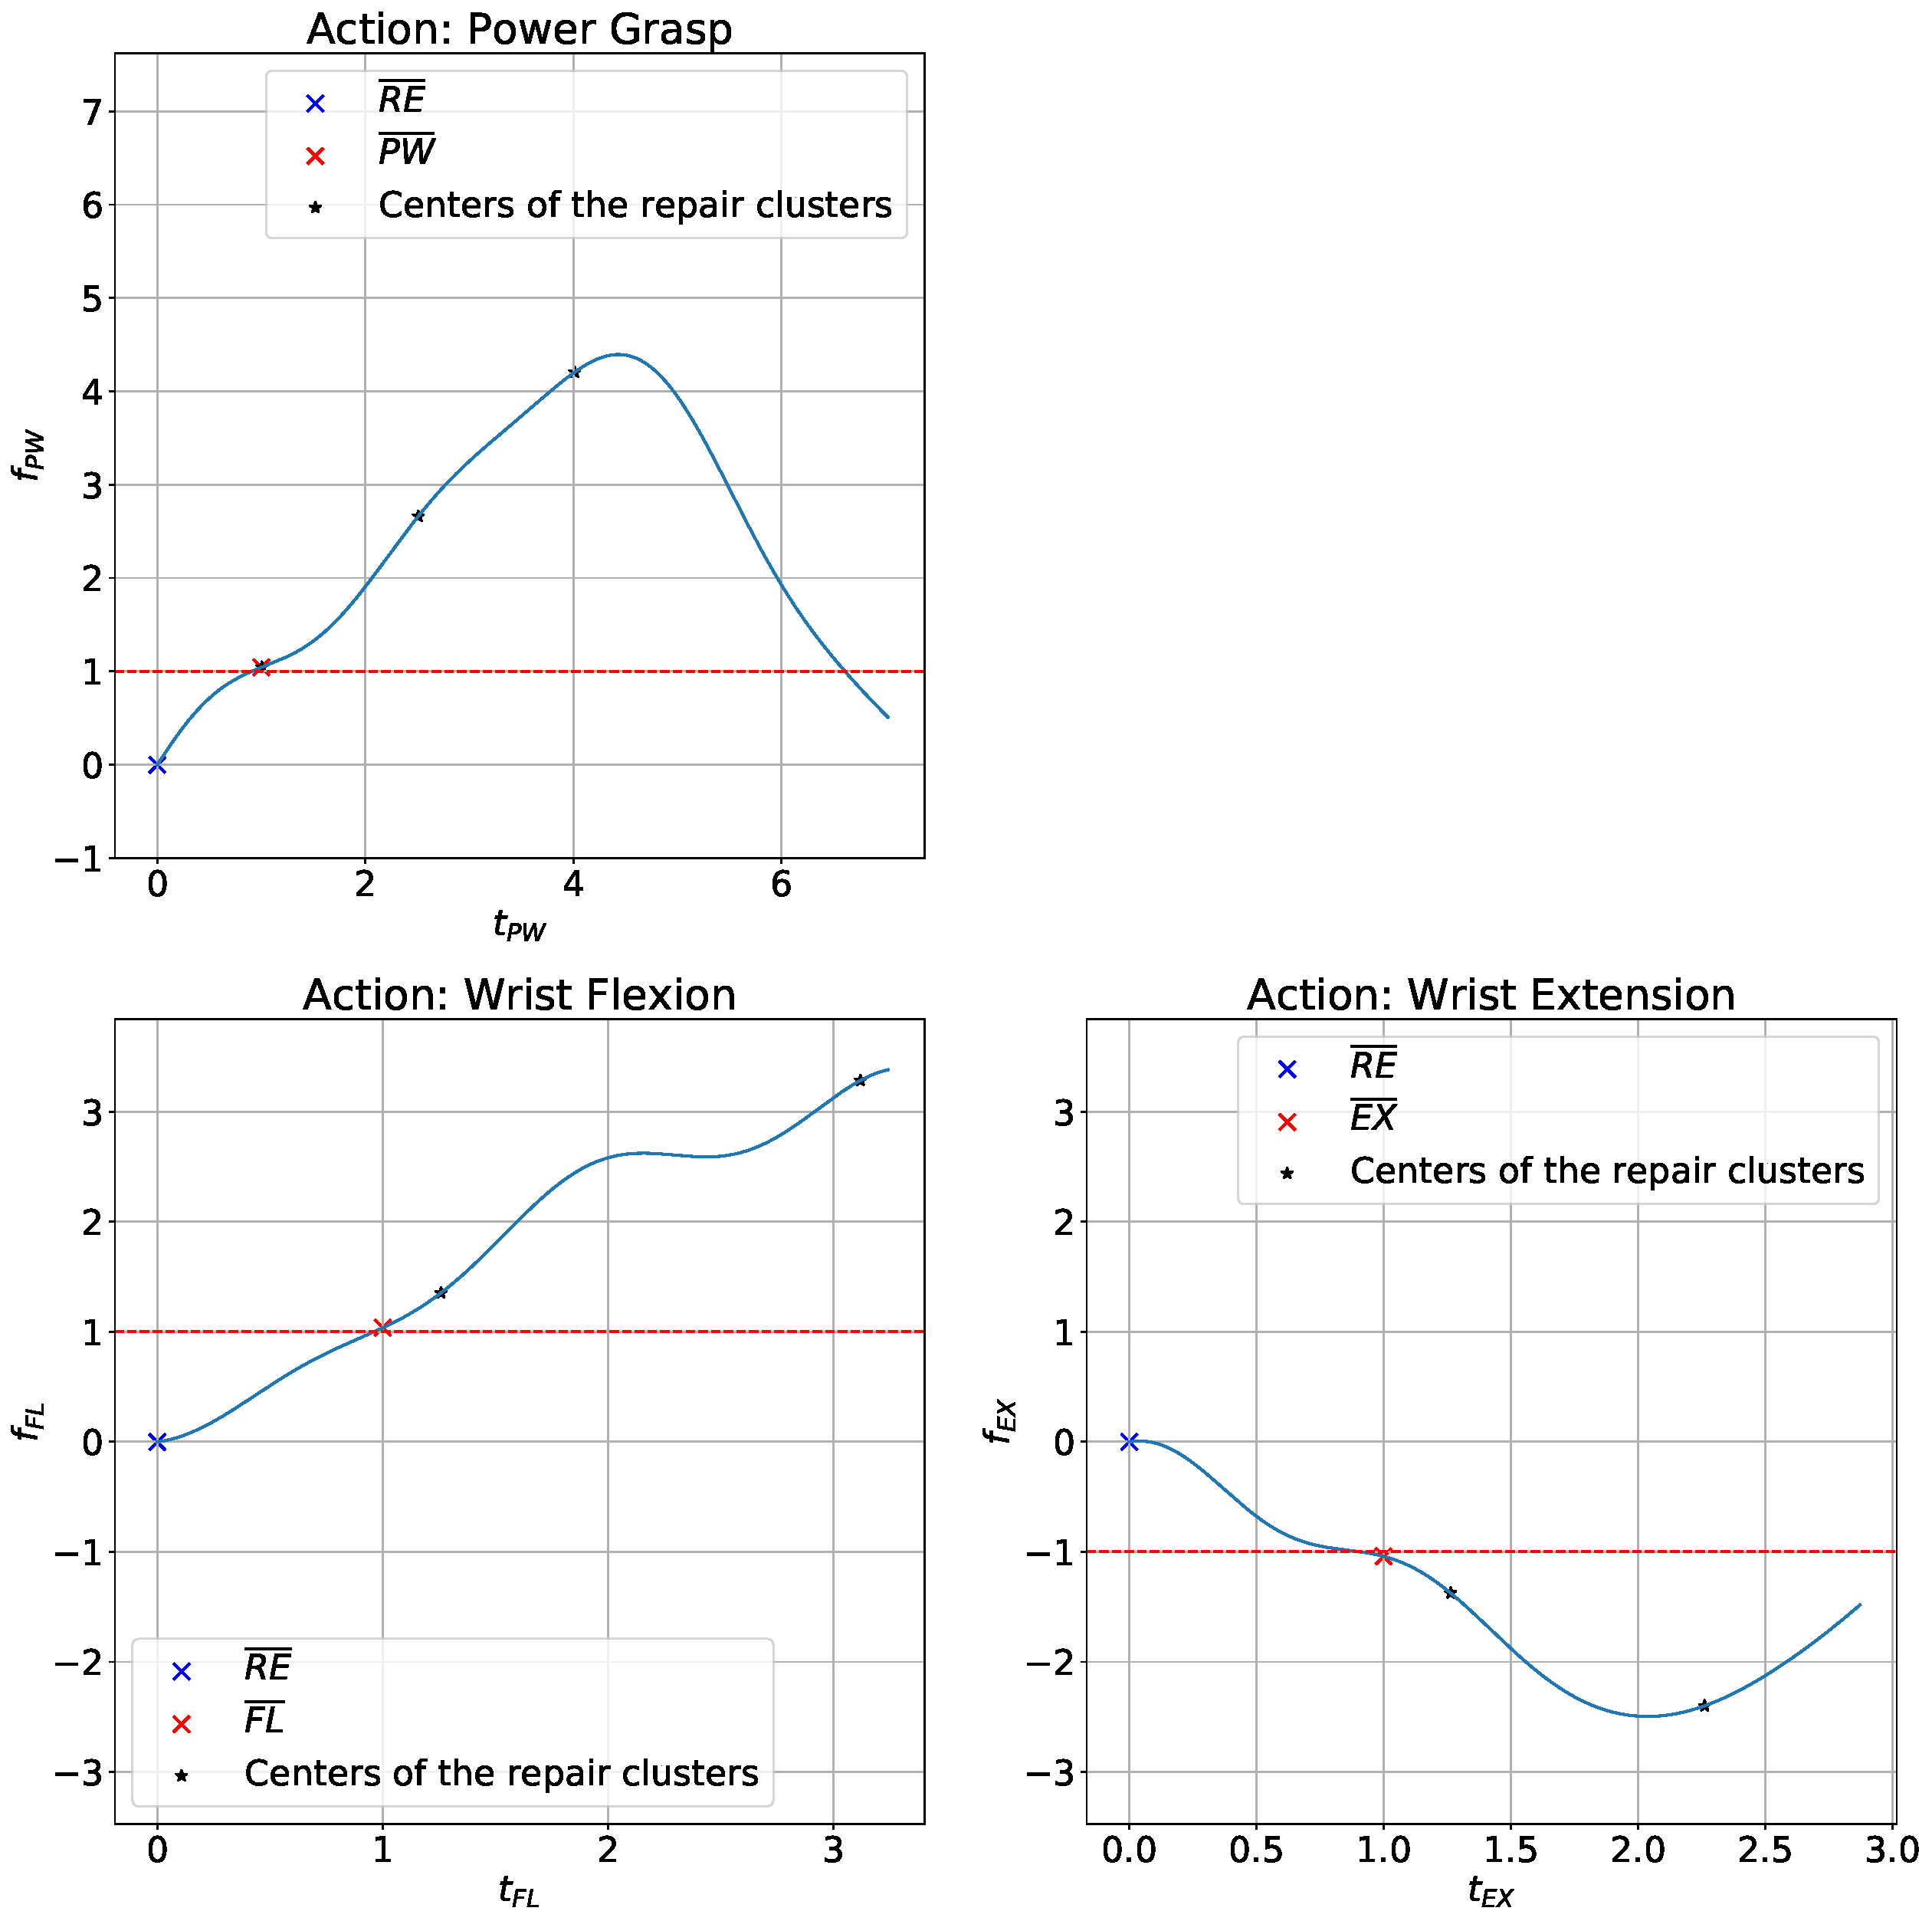
\includegraphics[width=\textwidth]{Images/repair-example/SMT-State3.pdf}
    \caption{In this figure we show the model along the straight lines $\overline{RE} + (\overline{PW} - \overline{RE})t_{PW}$, $\overline{RE} + (\overline{FL} - \overline{RE})t_{FL}$ and $\overline{RE} + (\overline{EX} - \overline{RE})t_{EX}$ after the third round of repair. The red dashed lines represent the maximum activation values for the different actions.}
    \label{fig:SMT-exec-3}
\end{figure}
\begin{figure}[H]
    \centering
    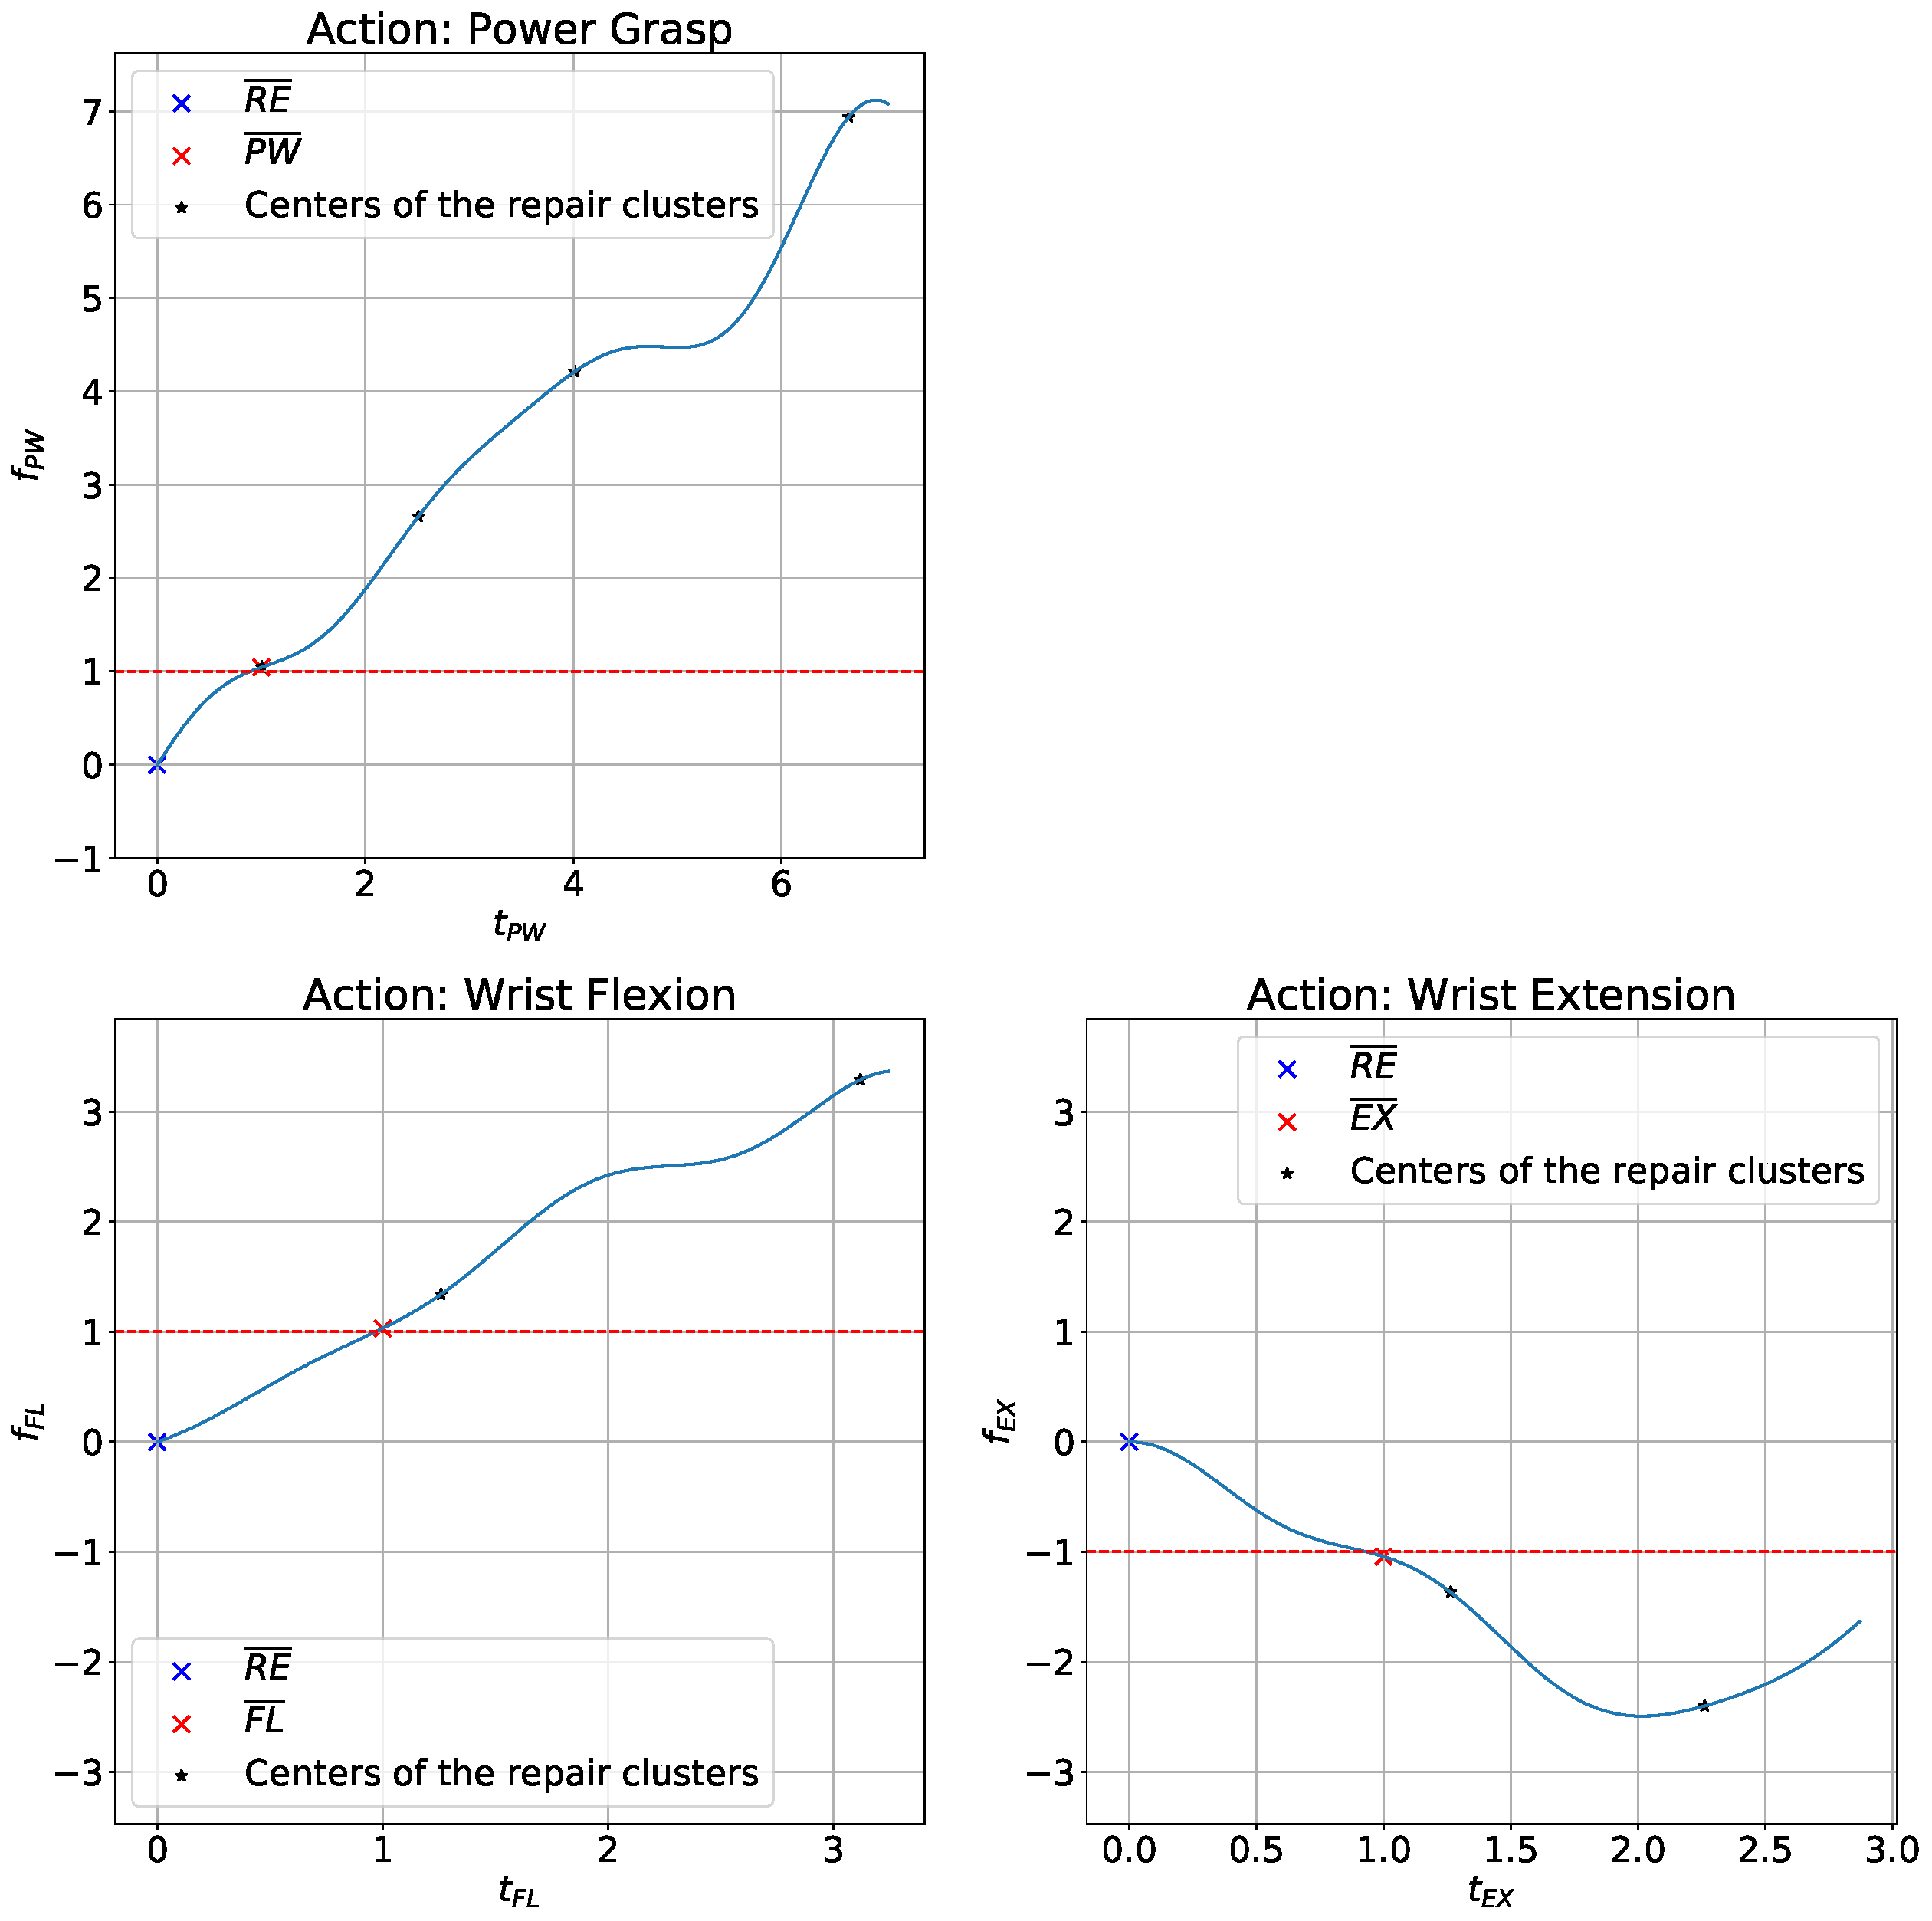
\includegraphics[width=\textwidth]{Images/repair-example/SMT-State4.pdf}
    \caption{In this figure we show the model along the straight lines $\overline{RE} + (\overline{PW} - \overline{RE})t_{PW}$, $\overline{RE} + (\overline{FL} - \overline{RE})t_{FL}$ and $\overline{RE} + (\overline{EX} - \overline{RE})t_{EX}$ after the final round of repair. The red dashed lines represent the maximum activation values for the different actions.}
    \label{fig:SMT-exec-4}
\end{figure}
As can be seen from the figures \ref{fig:PDO-exec-3} and \ref{fig:SMT-exec-4} the final results of the two repair procedures are quite similar and both manage to repair the process till the safety condition is verified (e.g. there are no unsafe points). From the graphs of the two executions can be easily seen one of the difference between the two repair process: since the PDO-Repair always search for the most unsafe points it is usually faster (e.g. require to generate less repair clusters). The other, and most important, difference between the two procedures is that the SMT-Repair guarantee the results to be correct accepting a one sided $\delta$-bounded error on the answer, where $\delta$ is a real positive number we can freely choose. Smaller value of $\delta$ corresponds to an higher computational complexity of the problem and therefore to a longer time necessary to complete the repair process; in particular what requires more time is the $\mathbf{safetyCheck(...)}$ procedure in which the SMT solver is used.
Even if we can guarantee a certain precision also for the PDO-Repair, increasing the number of points we use to analyse the straight lines, it is \textit{impossible to guarantee any level of precision} on the target values whereas the SMT-Repair guarantee a bound, given by $\delta$, on the answers of the SMT solver and therefore on the target values.
\begin{figure}[H]
    \centering
    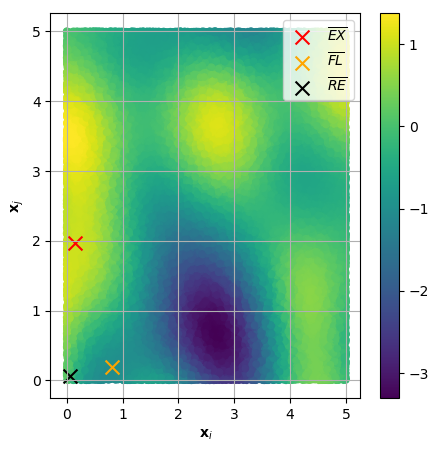
\includegraphics[width=0.45\textwidth]{Images/repair-example/SMT-2D-State0.png}
    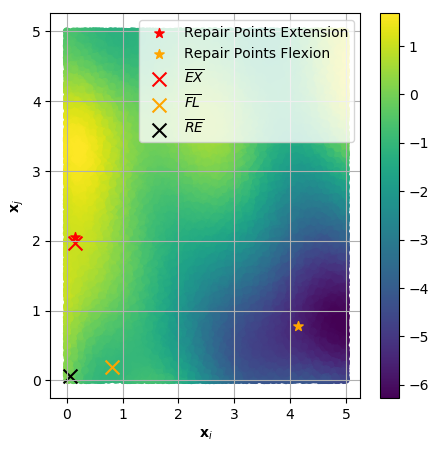
\includegraphics[width=0.45\textwidth]{Images/repair-example/SMT-2D-State1.png}
    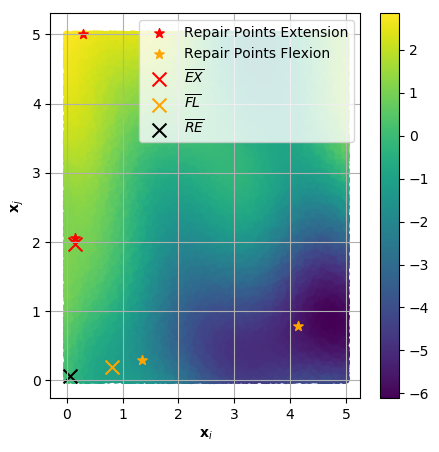
\includegraphics[width=0.45\textwidth]{Images/repair-example/SMT-2D-State2.png}
    \caption{In this figure we show the execution of SMT-Repair on a model built on a 2D-reduced exemplary dataset obtained after gathering observation for three actions (rest, RE; wrist flexion, FL; wrist extension, EX). We chose a 2D reduced dataset in order to be able to show the behaviour of the model on the whole input space.}
    \label{fig:SMT-exec-2D}
\end{figure}
Figure \ref{fig:SMT-exec-2D} shows that, even if our repair process explore only the subset of the input space represented from the straight lines of the type $\overline{RE} + (\overline{A} - \overline{RE})t_{A}$, the characteristics of the learning model guarantee a certain level of continuity which manage to extend the repairing also to the input space that it is not explicitly explored. This kind of generalisation, which we expect to be valid also for the full-dimensionality case, is the reason why the repair process manage to effectively enhance the reliability of the model in the real case, in which we are not only interested in the input space along the straight lines.
\chapter{Conclusion and Future Work}\label{c:conclusion}
HERE CONCLUSION

\bibliographystyle{abbrv}
\bibliography{mybib.bib}
\end{document}
